\graphicspath{{chapters/regularization}}
\chapter{Regularization of CCA Models to add Structure}\label{chap:als}
\minitoc
% chktex-file 44 
% chktex-file 3

\epigraph{All models are wrong, some are useful.}{\textit{G. Box}}
\section{Introduction}\label{sec:introduction}

This chapter explores the role of regularization in improving the performance and interpretation of Canonical
Correlation Analysis (CCA) using data from the Human Connectome Project (HCP) and Alzheimer's Disease Neuroimaging Initiative (ADNI) datasets.

CCA models often exhibit shortcomings when dealing with high-dimensional data.
This challenge is particularly acute in brain-behavior studies where the dimensionality of neuroimaging data is often orders of magnitude larger than the number of subjects.
In this context, CCA models are prone to overfitting, leading to spurious correlations and poor generalization.
Regularization, having been extensively studied and well-understood in the contexts of Linear Regression and Inverse Problems, introduces a deliberate bias to guide models towards more generalizable solutions.
This principle, when applied to CCA, offers a promising avenue for addressing its challenges, ensuring that the model does not overfit to the noise in the data but captures the true underlying patterns.
Furthermore, regularization can help us improve the interpretability of the results most clearly by encouraging sparsity.
However, due to the complexity of the CCA problem, regularization is not as straightforward as in Linear Regression.
The most popular approaches to `sparse CCA' have, in practice, been based on Partial Least Squares (PLS), which simplifies the optimization problem but, as we shall see, causes the model to inherit a bias towards the largest principal components from PLS.

With this perspective in mind, we propose a flexible regularized alternating least squares (FRALS) framework for CCA which allows us to incorporate any regularized least squares solver to efficiently implement a wide range of regularization functions, but in particular allows us to efficiently implement the elastic net penalty with controllable L2 and L1 penalties so that we can control the bias towards the largest principal components while still encouraging sparsity in the weights.
This is in contrast to much of the previous work on sparse Brain-Behavior analysis which has used a PLS objective with lasso constraints (SPLS), which inherits a bias towards the largest principal components from PLS.

We apply FRALS with ElasticNet regularization to Simulated Datasets as well as the Human Connectome Project (HCP) and Azlheimer's Disease Neuroimaging Initiative (ADNI) datasets.
We show that it outperforms other CCA models in terms of out-of-sample canonical correlation.
We also show that the identified mode of variation is distinct from previous work which identified latent variables with \gls{weights} related to cognitive tests and negatively related to cigarette, tobacco or alcohol\citep{smith2015positive}.
FRALS has stronger correlations with the Line Orientation test, which measures visuospatial abilities, and the parietal lobe, which is known to be involved in visuospatial processing.
This further demonstrates the importance of matching the model to the data generation process with the appropriate regularization.

This chapter expands on my work previously showcased at the OHBM conference and draws connections to a tutorial paper I co-authored, where I contributed a number of simulations\citep{mihalik2022canonical}.

\section{Background: Regularization for High-Dimensional and Structured Data}\label{sec:background}

Like Linear Regression, Canonical Correlation Analysis does not have a unique solution when the number of features exceeds the number of observations in either view.
More generally, as the number of features increases, the number of parameters in the model increases, and the model becomes more prone to overfitting particularly when the signal-to-noise ratio is low.
Furthermore, when features are correlated, the estimates of the parameters become unstable.
Most obviously, if two features are perfectly correlated, the model is not identifiable (has no unique solution) because we can swap the \gls{weights} between the two features without changing the model.
Regularization is a powerful tool for addressing these problems, and has been widely used in Linear Regression and Inverse Problems.
Moreover, regularization can help us improve the interpretability of the results by encouraging sparsity in the weights.

\subsection{Shrinkage Regularization}

Shrinkage regularization is an effective method for improving the performance of linear models in high-dimensional settings.
Shrinkage methods bias models towards lower variance solutions by shrinking the model parameters (weights) towards zero.
Shrinkage regularization works on the premise that, generally, larger principal components are more likely to represent meaningful data patterns rather than noise.

\paragraph{PLS as Shrinkage Regularization}

PLS can be interpreted as a form of shrinkage regularization applied to CCA. We can explain this by considering an analogy between CCA and \textit{Linear Regression} (indeed Linear Regression is a special case of CCA where \(X^{(2)}\) has one feature).

In Linear Regression, the ridge regression solution is given by:
\begin{align}
    \hat{\beta}_{\text{ridge}} = ((1-c)\Sigma_{X,X} + c I)^{-1} \Sigma_{X,y}
\end{align}
Where \(c\) is the regularization parameter between 0 and 1\footnote{It is more common to see $(\Sigma_{X,X} + c I)^{-1} \Sigma_{X,y}$ but these are equivalent up to a scalar factor and this form helps us later on}.
The ridge penalty acts in two important ways:
\begin{itemize}
    \item It shrinks the \gls{weights} towards zero.
    \item It biases the solution to high covariance directions rather than high correlation directions.
\end{itemize}

As $c$ becomes large, $\lim_{c \to \infty} (\Sigma_{X,X} + c I)^{-1} = (c I)^{-1}$
, so that $\hat{\beta}_{\text{ridge}}=\frac{\Sigma_{X,y}}{c}$, which is precisely the covariance of the features of $X$ with $Y$ scaled by $c$ (and shrunk towards zero for $c \geq 1$).
Notice that the ridge regression solution is no longer sensitive to the correlation of features in $X$.
Additionally, notice that for sufficiently large $c$, $(\Sigma_{X,X} + c I)$ is invertible even if $\Sigma_{X,X}$ is not invertible, so that ridge regression can be well defined even when the number of features exceeds the number of observations.

Now consider the CCA problem.
Firstly, recall that PLS and CCA are equivalent up to a scaling when the covariance matrices are identity matrices, a similar relationship to the relationship between Linear and Ridge Regression.
Consider the well-known form of CCA given in equation~\ref{eq:cca}\citep{mihalik2022canonical} (formed by reparameterizing \(u\sps{i}=(\Sigma_{ii})^{-\frac{1}{2}}u\sps{i}\)):

\begin{align}\label{eq:cca}
     & u_{\text{opt}}=\underset{u}{\mathrm{argmax}}\{ u\spstop{1}(\Sigma_{11}+ c I)^{-\frac{1}{2}}\Sigma_{12}(\Sigma_{22}+c I)^{-\frac{1}{2}}u\sps{2} \} \\
     & \text{subject to:} \notag \\
     & u\spstop{1}u\sps{1}=1, u\spstop{2}u\sps{2}=1 \notag
\end{align}

As we increase $c$, $\lim_{c \to \infty} (\Sigma_{ii}+ c I)^{-\frac{1}{2}}= (c I)^{-1}$ so that the objective approaches:

\begin{align}
     & u_{\text{opt}}=\underset{u}{\mathrm{argmax}}\{ u\spstop{1}(c I)^{-1}\Sigma_{12}(c I)^{-1}u\sps{2} \} \\
        & \text{subject to:} \notag \\
        & u\spstop{1}u\sps{1}=1, u\spstop{2}u\sps{1}=1 \notag
\end{align}

Which is precisely the PLS objective and constraints with an arbitrary scaling of the covariance matrix $\Sigma_{12}$ by $\frac{1}{c^2}$.
For this reason, we can consider PLS as a shrinkage method for CCA equivalent to adding a very large ridge regularization.
This has two important consequences.
Fortunately, it is well-defined even when the number of features exceeds the number of observations so we can always apply PLS to high-dimensional data.
Unfortunately, it biases the solution towards the largest principal components.
Although one would rarely resort to maximally regularized ridge regression except in extremely low sample sizes or high-dimensional data, it has become almost standard practice to use PLS in neuroimaging and genetics.
One of the core contributions of this chapter will be to demonstrate that PLS is usually a poor choice for regularization even in these very high-dimensional settings and that more nuanced regularization methods can offer significant improvements in performance and interpretability.
PLS is evidently not a nuanced tool for regularization because it offers no control over the degree of regularization applied.

\paragraph{Ridge Regularization}

For this reason,~\citet{vinod1976canonical} proposed the \textit{Canonical Ridge}, which combined the PLS and CCA constraints in a single constrained optimization:

\begin{align}
     & u\sps{1}_{\text{opt}} = \underset{u\sps{1}}{\mathrm{argmax}} \{ u\spstop{1} \hat{\Sigma_{12}} u\sps{2} \} \\
     & \text{subject to:} \notag \\
     & (1 - c_1) u\spstop{1} \hat{\Sigma_{11}} u\sps{1} + c_1 u\spstop{1} u\sps{1} = 1 \notag \\
     & (1 - \tau_2) u\spstop{2} \hat{\Sigma_{22}} u\sps{2} + \tau_2 u\spstop{2} u\sps{2} = 1 \notag
\end{align}

Where $c_1$ and $\tau_2$ are the ridge regularization parameters for the first and second views respectively.

\paragraph{PCA-CCA} PCA can be used as a regularization method for CCA by using only the first \( k \) principal components of each view as the input to CCA.
This reduces the dimensionality of the data and can help to avoid overfitting.
However, it also risks overlooking subtle but crucial relationships between variables, as it focuses on leading principal components.

While PCA-CCA and rCCA are effective for finding signal in the presence of noise, they do not produce sparse
solutions and so do not clearly lend themselves to interpretation.

\paragraph{A Visual Comparison of Shrinkage Techniques}

The distinct effects of Ridge and PCA on the eigenvalues of the effective covariance matrices can be clearly visualized with a simple visualisation.
We plot the eigenvalues of covariance matrices as perceived by models with different regularization techniques \footnote{e.g. the eigenvalues of $(1 - c_i) \hat{\Sigma_{ii}} + c_i I$ for ridge and $\hat{\Sigma_{ii}}$ truncated to include only the largest $k$ principal components for PCA}.
As shown in Figure~\ref{fig:shrinkage}, Ridge regularization reduces the magnitude of the largest eigenvalues in the effective covariance matrix towards 1, and increases the magnitude of the smallest eigenvalues towards 1.
On the other hand, PCA-CCA, leaves the largest eigenvalues unchanged, and ignores the smallest eigenvalues (we could have represented this by setting them to infinity).

\begin{figure}
    \centering
    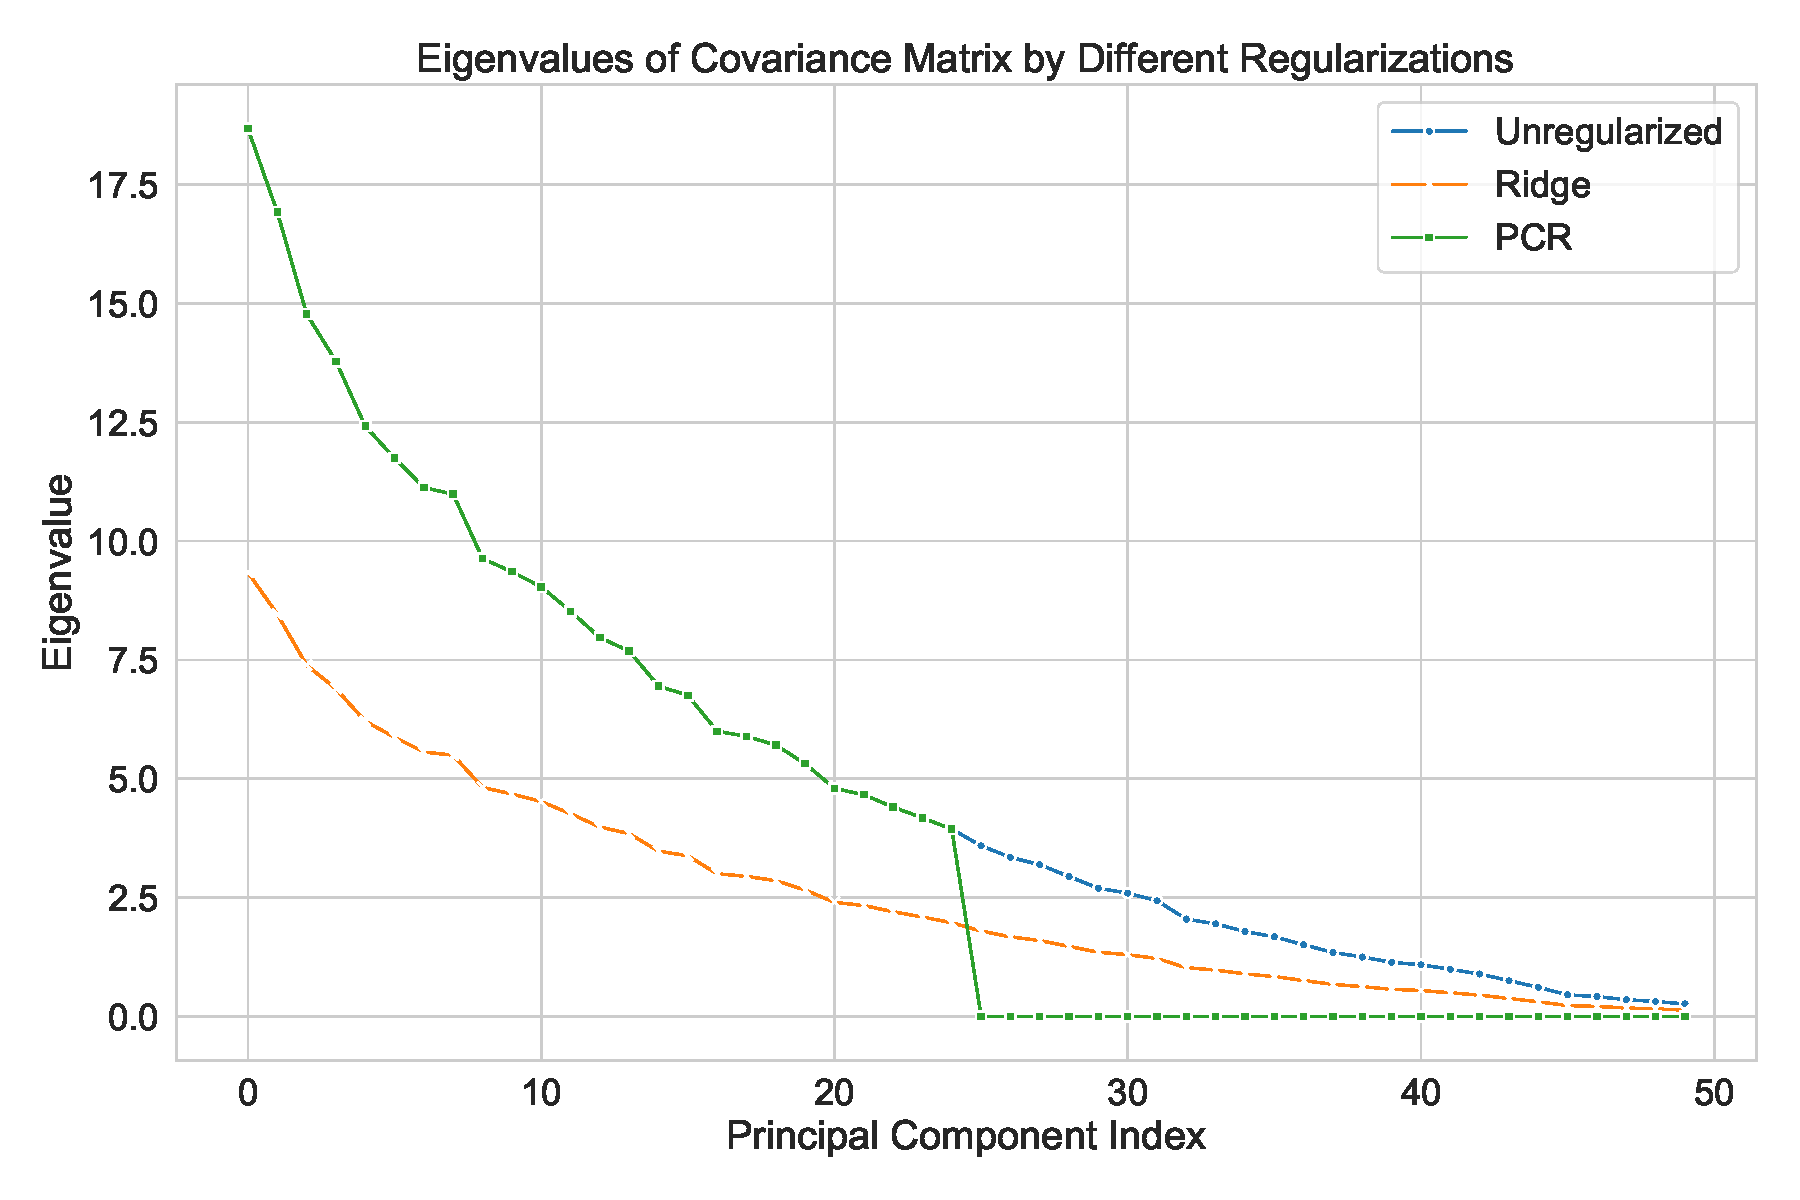
\includegraphics[width=0.8\textwidth]{figures/shrinkage/shrinkage}
    \caption{Comparison of the effect of OLS, Ridge, and PCA-CCA regularization on the eigenvalues of the covariance matrix.}\label{fig:shrinkage}
\end{figure}

When these effective covariance matrices are inverted to form the CCA objective, these effects are reversed.
Ridge regularization increases the magnitude of the weights associated with the largest eigenvalues and decreases the magnitude of the smallest eigenvalues.
PCA-CCA maintains the weights associated with the largest eigenvalues and sets the weights associated with the smallest eigenvalues to zero.
The visualization underscores the intrinsic nature of each regularization method:
\begin{itemize}
    \item \textbf{Unregularized}: Presents the unaltered spectrum, making it susceptible to noise but preserving potential subtle patterns.
    \item \textbf{Ridge}: Warps the spectrum, shrinking the largest eigenvalues and expanding the smallest eigenvalues, potentially missing subtle patterns but offering a cleaner representation of stronger associations.
    \item \textbf{PCA}: Truncates the spectrum, ignoring the smallest eigenvalues and preserving the largest eigenvalues, potentially missing subtle patterns but offering a cleaner representation of stronger associations.
\end{itemize}
The choice between these shrinkage techniques should in general be based on the nature of the data.
We now transition to another essential regularization technique: sparse regularization.
While shrinkage aims to prevent overfitting by pulling weight estimates towards zero to reduce variance, sparse regularization aims to set \gls{weights} to zero with the added benefit of enhancing model interpretability.

\subsection{Sparse Regularization}

Sparse regularization is a powerful tool for improving the performance and interpretability of linear models.
Sparse regularization encourages the model to use only a subset of the features, which can help to avoid overfitting and improve the interpretability of the model.
Sparse regularization works on the premise that only a subset of the features are relevant to the model.
Sparsity is typically achieved by adding either an L1 penalty or constraint\footnote{The L0 norm of the weight vector is the number of non-zero elements in the vector and is arguably a closer match to the goal, but the L0 norm is (a) not a proper norm in the mathematical sense and (b) not convex and so is difficult to optimize.}.
The L1 penalty is defined as:

\begin{align}
    \|u\|_1 = \sum_i |u_i|
\end{align}

Intuitively, this is the sum of the absolute values of the elements of the vector.
Now, with a foundational understanding of sparse regularization, we review a number of approaches to adding sparsity to the CCA problem.

\paragraph{Sparse PLS: Penalized Matrix Decomposition}
Penalized Matrix Decomposition (PMD)~\citep{witten2009penalized} provides an approximate solution to the sparse CCA problem by altering the constraints of the classical CCA formulation.
Specifically, PMD replaces the constraints \(u\spstop{i} \hat{\Sigma_{ii}} u\sps{i} = 1\) with the PLS constraints \(u\spstop{i} u\sps{i}= 1\) and additionally imposes \(\|u\spstop{i}\|_1 \leq \tau\).
The optimization problem for PMD is then given by:

\begin{align}
    & u^{opt}=\underset{u}{\mathrm{argmax}}\{ u\spstop{1} \hat{\Sigma_{12}} u\sps{2} \} \\
    & \text{subject to:} \notag \\
    & u\spstop{1} u\sps{1} = 1 , u\spstop{2} u\sps{2} = 1 \notag \\
    & \|u\sps{1}\|_1 \leq \tau_1 , \|u\sps{2}\|_1 \leq \tau_2 \notag
\end{align}

This Sparse PLS (SPLS) approximation has been highly influential as a form of Sparse CCA because it is extremely efficient method \footnote{it can be solved by a variant of the power method; iteratively multiplying $u\sps{1}$ by $\hat{\Sigma_{12}}$ and soft-thresholding}.
There are a number of other sparse CCA methods that employ the PLS approximation\citep{parkhomenko2009sparse, waaijenborg2008quantifying, lindenbaum2021l0}.
However, while the PLS approximation is efficient, it means these methods inherit a bias towards the largest principal components from PLS.

To address these problems and truly tackle the sparse CCA optimization, another class of approaches have adopted a penalized least squares approach.

\paragraph{Sparse CCA: Least Squares Approaches}

It is well known that the CCA problem can be formulated as a constrained least squares problem with the intuition that
for \(X\sps{1} u\sps{1}=1\) and \(X\sps{2} u\sps{2}=1\), correlation is maximized when the squared distance
between \(X\sps{1} u\sps{1}\) and \(X\sps{2} u\sps{2}\) is minimized. \citep{golub1995canonical} proved the
convergence of a simple algorithm which alternates between solving the least squares problem for \(u\sps{1}\) and
\(u\sps{2}\) while keeping the other fixed.

With this intuition, \cite{wilms2015sparse} and \cite{mai2019iterative} separately proposed iterative penalized least
squares methods for sparse CCA\@.

\begin{align}
    \label{eq:mai}
    u^{opt} &= \underset{u}{\mathrm{argmin}} \left\{ \|X\sps{1}u\sps{1} - X\sps{2}u\sps{2}\|_2^2 + P(u) \right\} \\
    &\text{subject to:} \notag \\
    &u\spstop{1} \hat{\Sigma_{11}} u\sps{1}=1 \notag \\
    &u\spstop{2} \hat{\Sigma_{22}} u\sps{2}=1 \notag
\end{align}

Where \(P(u)\) is a penalty function.
The penalty term can be any function that penalizes the norm of the vector \(u\).
\citep{mai2019iterative} proved that solving the subproblems where one of $u\sps{i}$ is fixed is easy for one-homogenous $P$ where
\( P((\mu + 1)\theta) = (\mu + 1)P(\theta) \) which notably includes the lasso penalty.
This means a sparse CCA based
on alternating lasso regressions can be solved relatively efficiently using existing solvers.
However, the one homogenous penalty in practice limits the flexibility of the method.
For example, the elastic net penalty is not one-homogenous and therefore cannot be used with this method.
\citet{6556581} and \cite{Mullins2021} added ridge penalties to the subproblems to improve the conditioning of the problem in a way that could be considered a form of elastic net regularization but the subproblems no longer correctly optimize the global objective\footnote{when rescaling the penalized solutions back to unit variance}.

\paragraph{Sparse CCA: Proximal Gradient Descent and ADMM}
\citet{kanatsoulis2018structured} proposed solving equation~\ref{eq:mai} for more general classes of $P$ using the alternating direction method of multipliers (ADMM)~\citep{boyd2011distributed}.
\cite{fu2017scalable} propose a regularized CCA based on an alternative classical CCA formulation, sometimes called the MAXVAR formulation, which views the problem as a constrained least squares with an auxiliary representation $T$\citep{carroll1968generalization,kettenring1971canonical}.

\begin{align}\label{eq:fu}
    \underset{U, T}{\mathrm{argmin}}\left\{\sum_i \|X\sps{i} U\sps{i} - T\|_F^2\right\}\\
    \text{subject to: }T^\top T = I\\
\end{align}

In this formulation, \(U\sps{i}\) represents the \gls{weights} for the $i^{\text{th}}$ view, and \(T\) denotes the latent variable matrix.
The premise is that when \(T\) closely mirrors \(X\sps{i} U\sps{i}\) across all \(i\), the scores correlate.
Notably, this method is adaptable to multiple views.
The authors employed proximal gradient descent for regularization, specifically suited for penalties like the lasso.
While these methods are flexible, they don't have the plug-and-play nature of the penalized least squares methods.
Not just a matter of convenience, this means that these methods are not compatible with existing solvers for regularized least squares problems like for example total variation regularisation solvers in nilearn, which are often highly optimized for specific problems and modalities.

Having discussed the benefits of both shrinkage (e.g., PCA-CCA, Ridge CCA, PLS) and sparsity (SPLS, Sparse CCA) in handling high-dimensional, noisy data, a natural progression is to integrate these advantages.
Specifically, the challenge lies in fusing shrinkage and sparsity within the CCA framework, enhancing the interpretability and performance of Brain-Behaviour association models.
The solution?
A method that employs readily available regularized regression solvers, allowing for flexible and tunable regularization in CCA.
This leads us to introduce the Flexible Regularized Alternating Least Squares (FRALS).
\newpage
\section{Methods}

In this section, we outline the methodologies employed in our study for Canonical Correlation Analysis (CCA) and related techniques.
We first introduce the Flexible Regularized Alternating Least Squares (FRALS)—a versatile solution to the regularized CCA problem that incorporates various regularization functions, notably the elastic net penalty\citep{zou2005regularization}.
We then outline our experimental design, which assesses the performance of FRALS and other CCA variants, aiming to understand the effects of regularization on model performance and clarity.
Lastly, we specify the parameters and sources of the datasets used.

\subsection{Flexible Regularized Alternating Least Squares (FRALS)}\label{subsec:flexible-regularized-alternating-least-squares-(frals)}

The primary goal of our Flexible Regularized Alternating Least Squares (FRALS) framework is to provide a versatile and user-friendly interface for Canonical Correlation Analysis (CCA). This is achieved by designing the framework to be compatible with any scikit-learn compatible regularized least squares solver. This compatibility is pivotal as it allows researchers and practitioners to leverage the extensive range of solvers available in scikit-learn, a popular machine learning library in Python.

This approach marks a significant departure from traditional methodologies in CCA, which often focused on developing or utilizing specific solvers tailored for particular types of data or computational constraints. By contrast, our FRALS framework democratizes access to advanced CCA techniques, allowing users to select solvers that best fit their specific data characteristics, computational needs, or familiarity. Such flexibility is particularly advantageous in interdisciplinary fields like neuroimaging, where diverse datasets and varying levels of technical expertise are common.

For example, users dealing with high-dimensional, sparse neuroimaging data could opt for solvers optimized for such datasets, while those needing parallel computation for large data sets might choose solvers with GPU acceleration capabilities.
In principle, FRALS can even be used with Neural Network-based solvers, which are becoming increasingly popular in machine learning\footnote{Though for reasons that will later become clear, we do not reccommend this!}.
This adaptability enhances FRALS' accessibility and future-proofs the framework against evolving computational technologies and data analysis needs.

In the technical implementation of FRALS, we consider the formulation for a single latent variable \(t\) with regularization \(\lambda_i P_i\) on the weights \(u^{(i)}\):

\begin{align}
    \underset{u}{\mathrm{argmin}}\left\{\sum_i \|X^{(i)} u^{(i)} - t\|_2^2 + \textcolor{red}{\lambda_i P_i(u^{(i)})} \right\}\\
    \text{subject to: }t^\top t = 1\\
\end{align}

This problem can be decomposed into three subproblems. The first subproblem for the auxiliary variable \(t\):

\begin{align}
    \underset{t}{\mathrm{argmin}}\left\{\sum_i \|X^{(i)} u^{(i)} - t\|_2^2\right\}\\
    \text{subject to: }t^\top t = 1\\
\end{align}

is a standard least squares problem and can be solved in closed form by averaging \(X^{(i)} u^{(i)}\) and normalizing. This makes \(t\) an estimate of the latent variables, as recalled from section~\ref{subsec:generative-perspectives-on-cca}.

The subproblems for the weights \(u^{(i)}\):

\begin{align}
    \underset{u^{(i)}}{\mathrm{argmin}}\left\{\|X^{(i)} u^{(i)} - t\|_2^2 + \textcolor{red}{\lambda_i P_i(u^{(i)})} \right\}\\
\end{align}

are regularized least squares problems that can be solved using any suitable regularized least squares solver.

In this work, we employ the well-tested Elastic Net solver from the \texttt{scikit-learn} package~\citep{pedregosa2011scikit}, where \(P_i = \alpha_i \times \text{l1\_ratio} \|u^{(i)}\|_1 + \alpha_i \times (1-\text{l1\_ratio}) \|u^{(i)}\|_2^2\), allowing for independent tuning of shrinkage and sparsity of the weights.

In summary, the FRALS framework represents a paradigm shift in CCA methodologies, offering a more inclusive and adaptable approach to multivariate data analysis, aligning with the dynamic nature of research in fields like neuroimaging and beyond.

\subsection{The predictive framework for CCA}\label{subsec:the-predictive-framework-for-cca}

To evaluate the performance of CCA models, we employ a standard predictive framework.
We split the data into training and test sets using a 80:20 split, and use the training set to fit the model.
We then use the test set to evaluate the model's performance.
Where relevant, pre-processing is performed on the training set and the same pre-processing is applied to the test set.
This is important to avoid data leakage, where information from the test set is used to fit the model.

\subsubsection{Model Selection}

For the models that require hyperparameter tuning, we use a grid search to find the best hyperparameters.
Specifically, we use 5-fold cross-validation to evaluate the performance of a model with a given set of hyperparameters on 5 different splits of the training data with non-overlapping validation sets.
We optimise for the hyperparameters that give the best average out of sample correlation.

\subsubsection{Model Comparisons}
We employ several CCA variants for this experiment, including Canonical Correlation Analysis (CCA), Partial Least Squares (PLS), and more.

\begin{table}[h]
\centering
\caption{Employed CCA Variants}
\begin{tabular}{|l|l|l|l|}
\hline
\textbf{Model} & \textbf{Abbreviation} & \textbf{Hyperparameters}  \\
\hline
Canonical Correlation Analysis & CCA & -   \\
\hline
Regularized CCA & RCCA & \(c_1, c_2\)   \\
\hline
Partial Least Squares & PLS & -   \\
\hline
Sparse PLS & SPLS & \(\tau_1, \tau_2\)   \\
\hline
FRALS - Elastic & Elastic & \(\alpha_1, \alpha_2, \text{l1}_1, \text{l1}_2\)   \\
\hline
Principal Component Analysis & PCA & -  \\
\hline
\end{tabular}\label{table:cca-variants}
\end{table}

\subsection{Datasets}\label{subsec:datasets}

The datasets employed in our experiments comprise the HCP and ADNI data.
These datasets provide insights into brain functionality and behavior from different perspectives.
We chose the HCP and the ADNI datasets based on 2 recent landmark studies and the tutorial paper this chapter is loosely related to \cite{mihalik2022canonical}.

\subsubsection{The Human Connectome Project (HCP)}

The Human Connectome Project (HCP) offers publicly available resting-state functional MRI (rs-fMRI) and non-imaging measures like demographics, psychometrics, and other behavioral measures.
Specifically, we sourced data from 1003 subjects out of the 1200-subject data release of the HCP.
This dataset is constructed using brain connectivity features of the thoroughly processed rs-fMRI data.
This processing results in 19,900 brain connectivity variables for every subject.
Additionally, there are 145 non-imaging measures employed.
Notably, nine confounding variables were regressed out from both data modalities.
Each variable was standardized for zero mean and unit variance.
More details can be found in \cite{smith2015positive, mihalik2022canonical}.
We summarize the parameters of the HCP data in table~\ref{tab:hcp-parameters}.

\begin{table}
\centering
\caption{HCP Data Parameters}
\begin{tabular}{| l | l |}
\hline
\textbf{Parameter} & \textbf{Value} \\
\hline
Number of samples (\textit{n}) & 1003 \\
Number of features in View 1 (\textit{p}) & 19900 \\
Number of features in View 2 (\textit{q}) & 145 \\
\hline
\end{tabular}\label{tab:hcp-parameters}
\end{table}

\subsubsection{The Alzheimer's Disease Neuroimaging Initiative (ADNI)}

The ADNI database is found at \url{adni.loni.usc.edu}.
Launched in 2003, ADNI's main objective is to assess the combination of serial MRI, PET (Positron emission tomography), biological markers, and clinical and neuropsychological assessment in tracking the progression of Mild Cognitive Impairment (MCI) and early Alzheimer’s disease.
For our experiments, we used a subset of 592 unique subjects from the ADNI. The MRI scans underwent a series of processing stages, yielding a grey matter probability map
The Mini-Mental State Examination (MMSE) scores were employed to investigate the association with the grey matter maps.
Composed of a series of brief tasks, the MMSE evaluates various cognitive domains including memory, attention, language, and visuospatial skills.
The MMSE is a widely used test for assessing cognitive impairment.
The MMSE scores range from 0 to 30, with lower scores indicating more severe cognitive impairment.
We summarize the parameters of the ADNI data in table~\ref{tab:adni-parameters}.

\begin{table}
\centering
\caption{ADNI Data Parameters}
\begin{tabular}{| l | l |}
\hline
\textbf{Parameter} & \textbf{Value} \\
\hline
Number of samples (\textit{n}) & 592 \\
Number of features in View 1 (\textit{p}) & 168130 \\
Number of features in View 2 (\textit{q}) & 31 \\
\hline
\end{tabular}\label{tab:adni-parameters}
\end{table}

\newpage
\newpage
\section{Results}

\subsection{Human Connectome Project (HCP) Data}

Next, we consider the results of applying the various CCA variants to the HCP data.
Since the HCP data is high-dimensional, we drop CCA from the analysis since it would produce random results.

\subsubsection{Out of Sample Correlation}

The Elastic Net did not improve upon Ridge CCA in terms of holdout correlation captured (Figure~\ref{fig:performance}).
However, both Ridge CCA and ElasticNet outperformed PLS and SPLS.
This suggests that tunable L2 regularization is important, even for very high-dimensional data.
SPLS does however outperform PLS.

\begin{figure}
\centering
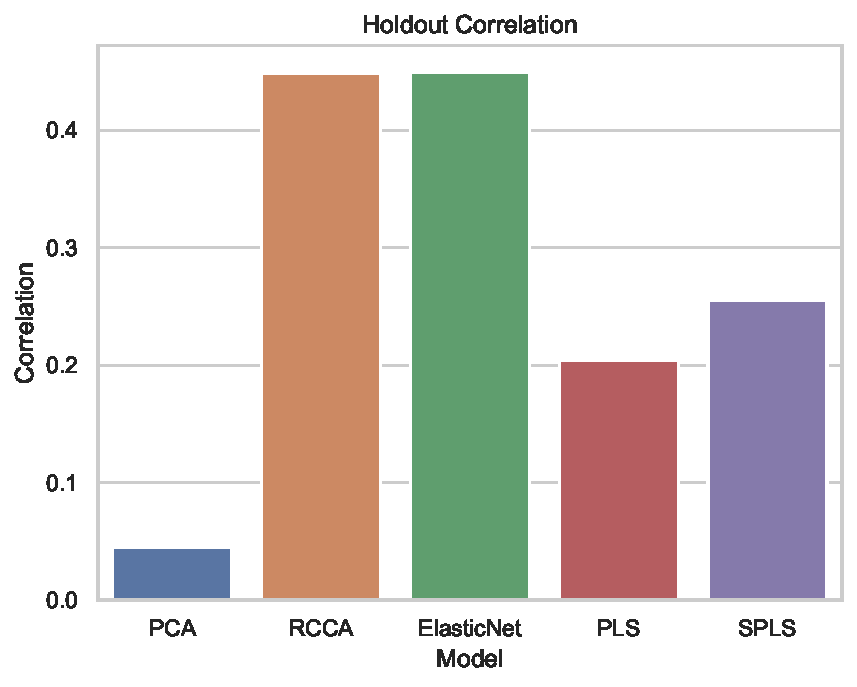
\includegraphics[width=0.5\linewidth]{figures/hcp/holdout_correlations}
\caption{Out-of-sample canonical correlations for each model.}
\end{figure}

\subsubsection{Behaviour Weights}

Figure\ref{fig:behaviour} plots the top 8 positive and negative non-imaging \gls{weights} for each model.
This is to illustrate some of the effects we have observed in the previous section.
PCA finds a mode of variation in the behavioural data that is positively correlated with psychiatric and life function tests and negatively correlated with a number of emotion and personality tests.
The RCCA and ElasticNet models find a mode of variation in the behavioural data that is negatively correlated with the Line Orientation test and to a lesser extent smoking and positively correlated with a number of other cognitive tests.
The PLS model finds a mode of variation in the behavioural data that is somewhat similar to the `positive-negative' mode in \cite{smith2015positive} with a positive correlation with agreeableness, vocabulary tests, and feelings about ones' life and a strong negative correlation with smoking, rule-breaking, and antisocial personality traits.
The SPLS mode is similar but selects out the rule-breaking and antisocial personality traits in favour of the vocabulary tests and smoking.

\begin{figure}
\centering
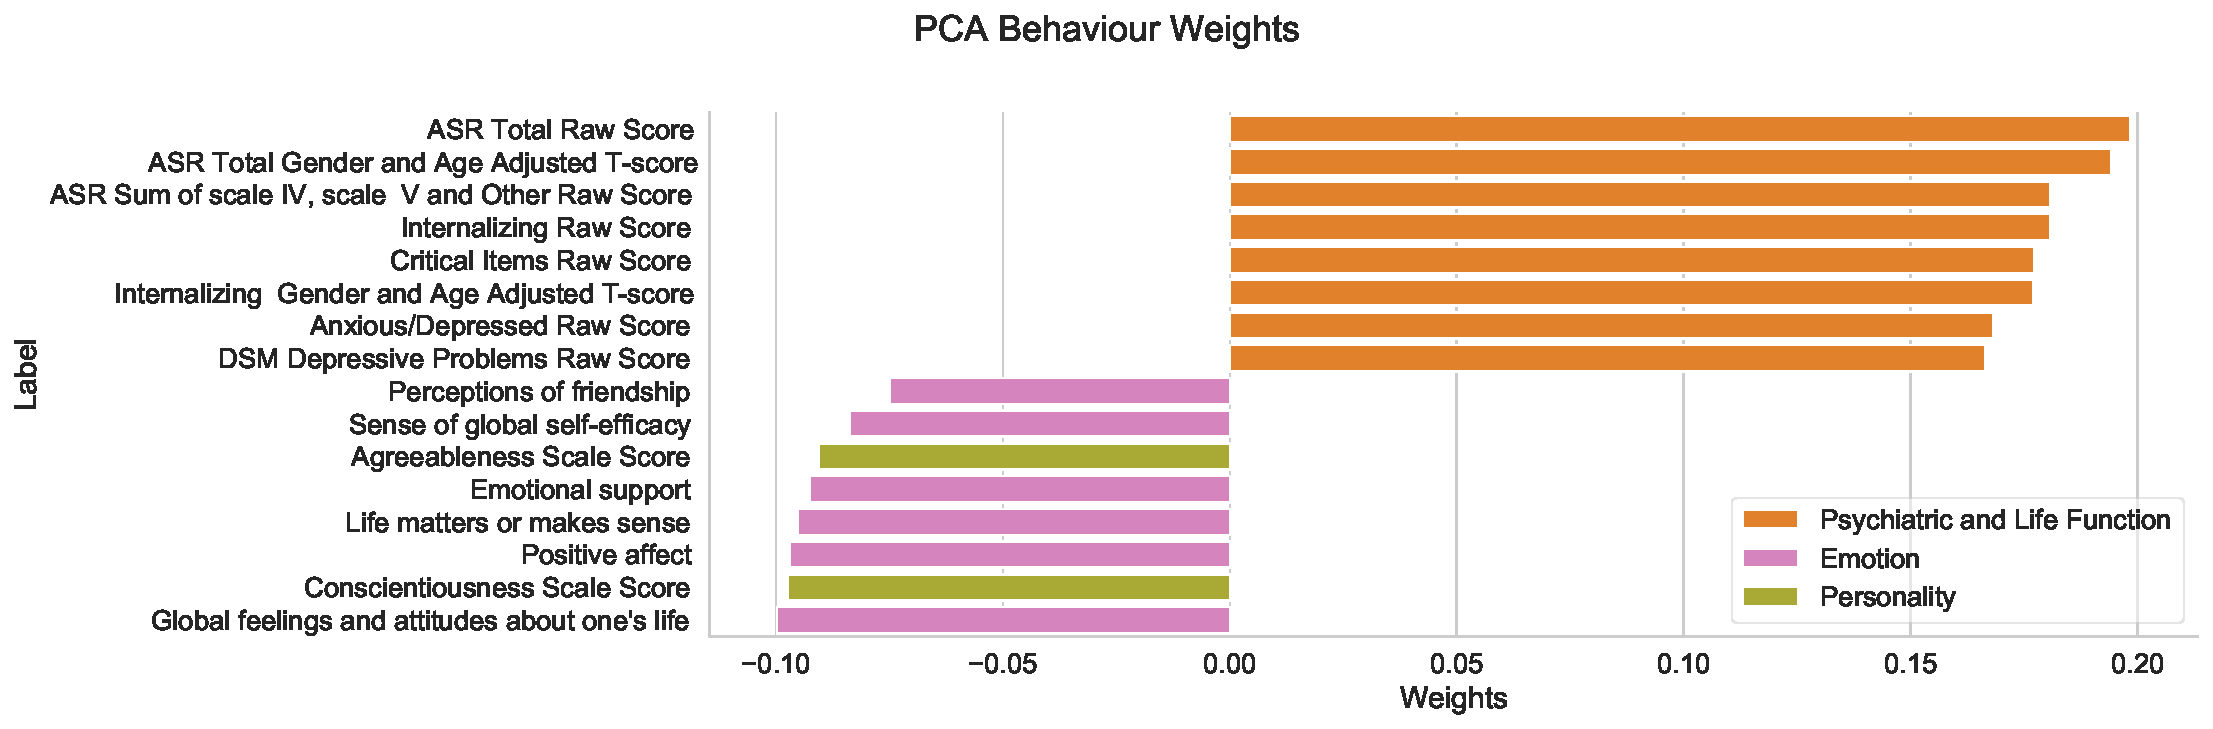
\includegraphics[width=0.8\linewidth]{figures/hcp/PCA behaviour weights}
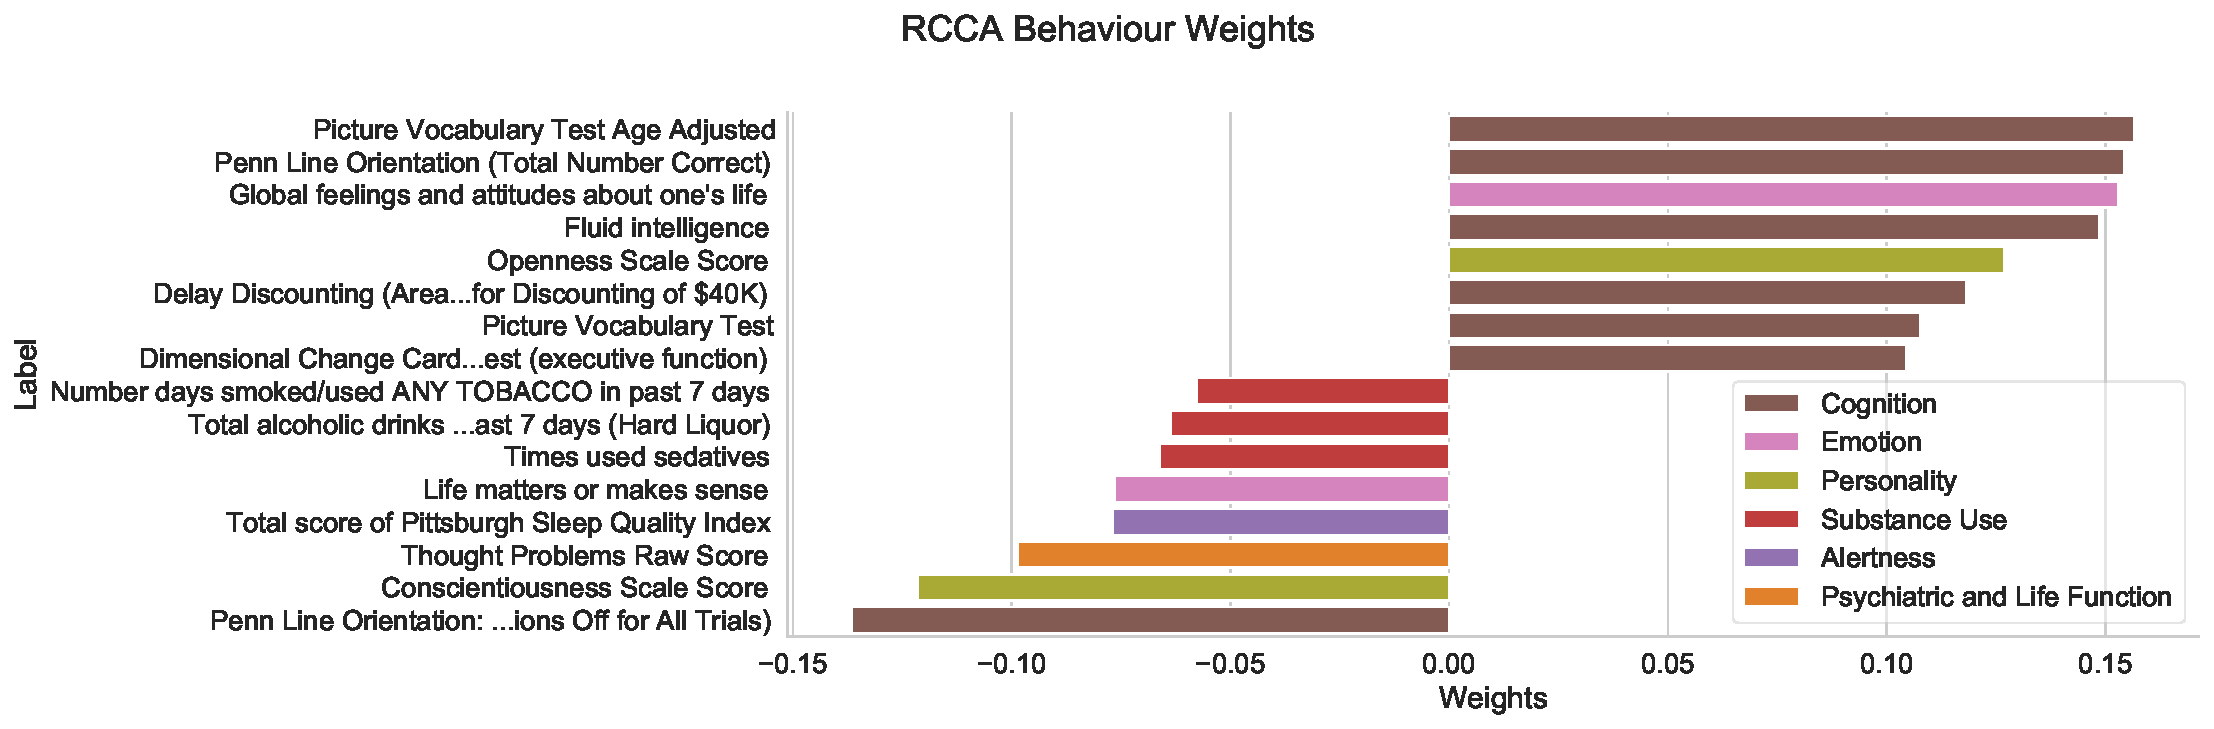
\includegraphics[width=0.8\linewidth]{figures/hcp/RCCA behaviour weights}
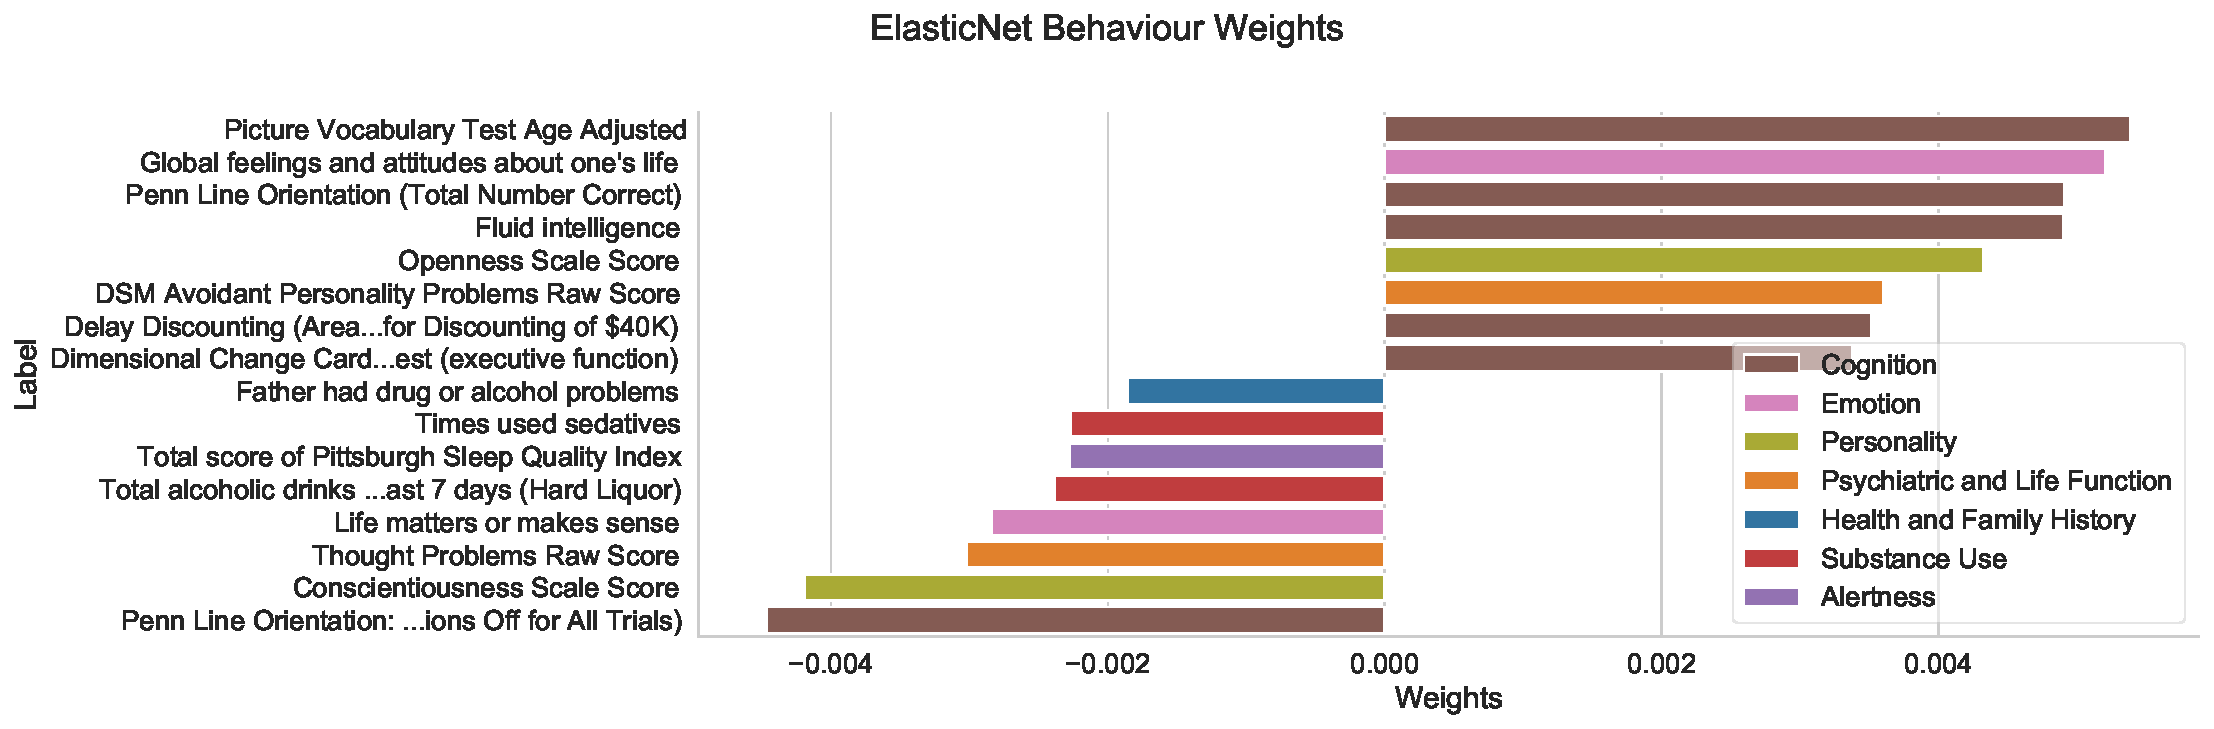
\includegraphics[width=0.8\linewidth]{figures/hcp/ElasticNet behaviour weights}
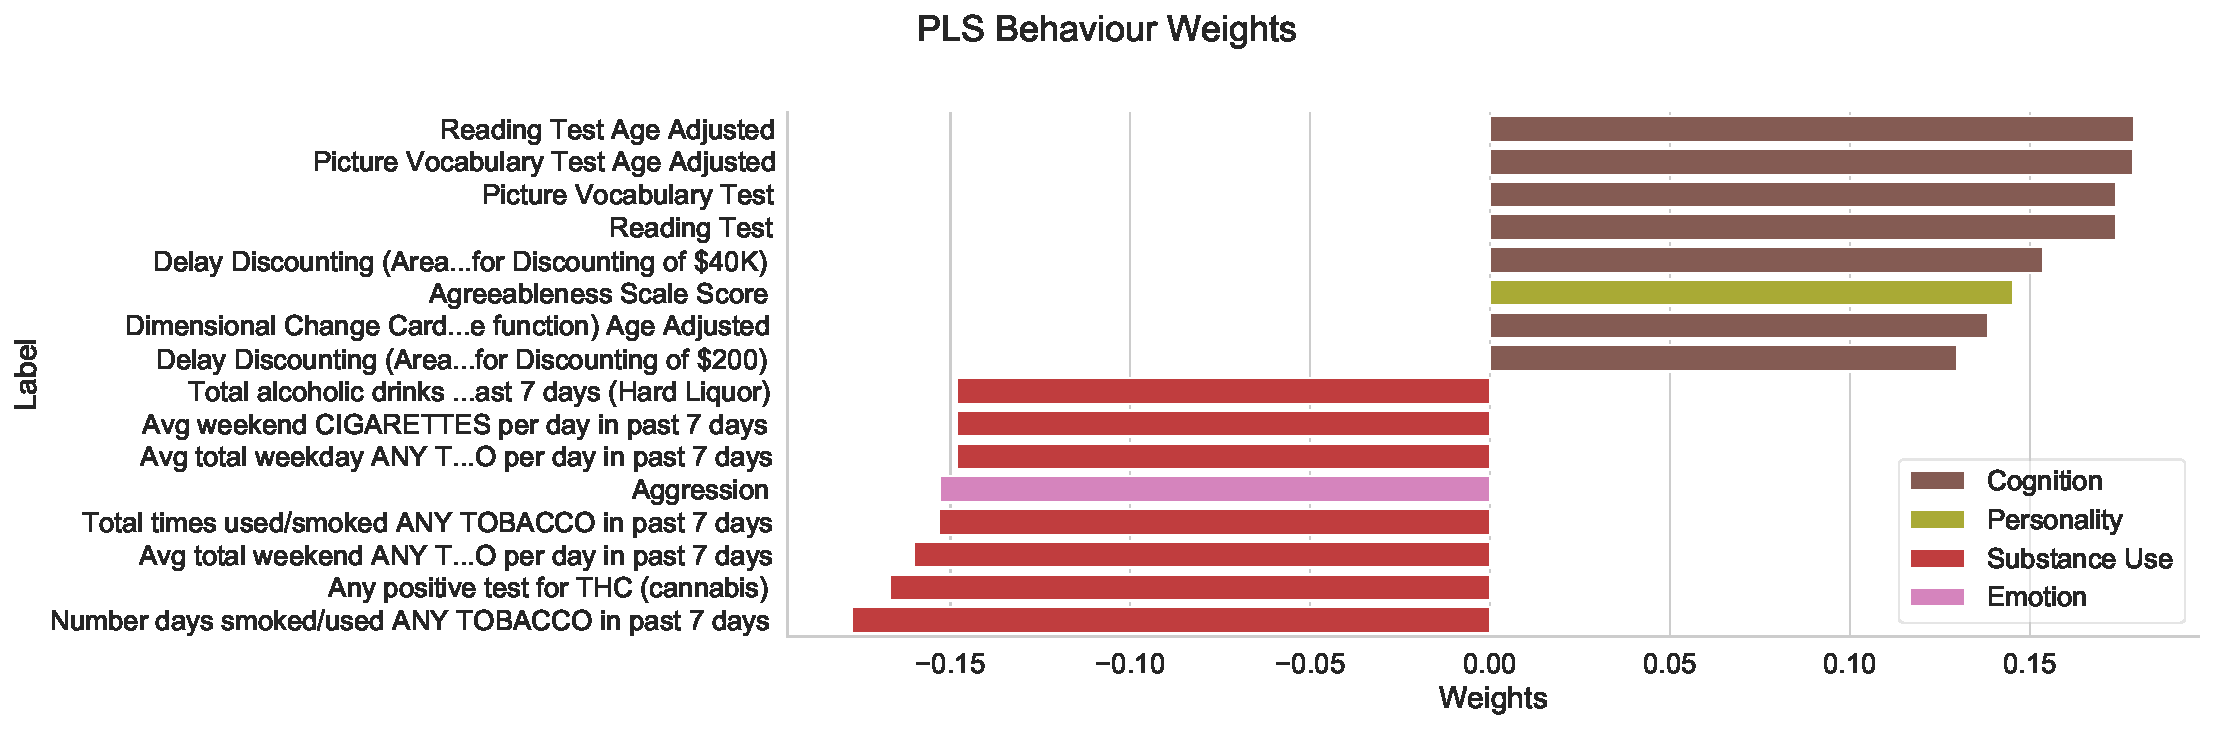
\includegraphics[width=0.8\linewidth]{figures/hcp/PLS behaviour weights}
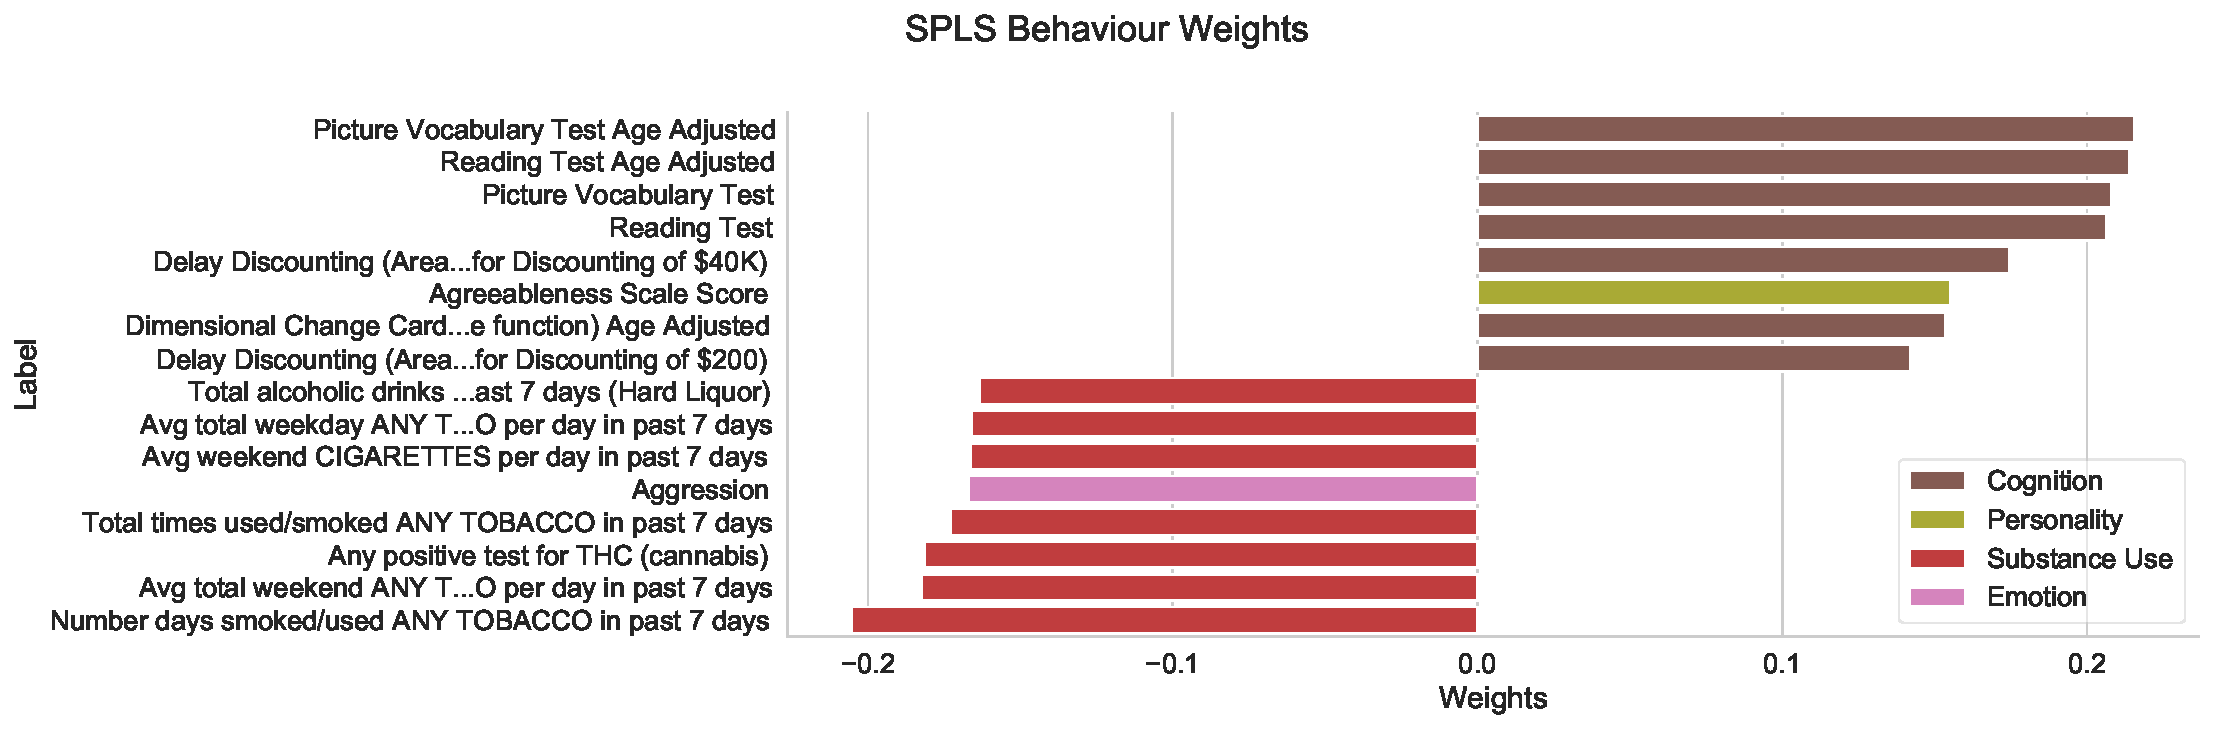
\includegraphics[width=0.8\linewidth]{figures/hcp/SPLS behaviour weights}
\caption{Top 8 positive and negative non-imaging \gls{weights} for each model}\label{fig:behaviour}
\end{figure}

\subsubsection{Brain Connectivity Weights}

In this section, we use two different methods to visualize the brain connectivity weights.
The first method is to use chord diagrams to visualize the top 8 positive and negative brain \gls{weights} for each model.
This approach is inspired by the chord diagrams used in \cite{smith2015positive}.
The second method is to use surface maps to visualize the brain connectivity weights.
This approach has been used by both \cite{ferreira2022hierarchical} and \cite{smith2015positive}.

\paragraph{Chord Diagrams}
We grouped the nodes of the connectivity matrix of our data into 7 parcels according to the Yeo 7 network parcellation \cite{yeo2011organization}.
These are then arranged around the circumference of the chord diagram using the Nichord package\citep{bogdan2023connsearch}.
The plots then show the 8 strongest positive and negative \gls{weights} for each model as `chords'.
The chord diagrams in Figure~\ref{fig:chord_weights} show the top 8 positive and negative brain \gls{weights} for each model.

\textcolor{red} Need to find something biologically useful to say about these.

\begin{figure}
\centering
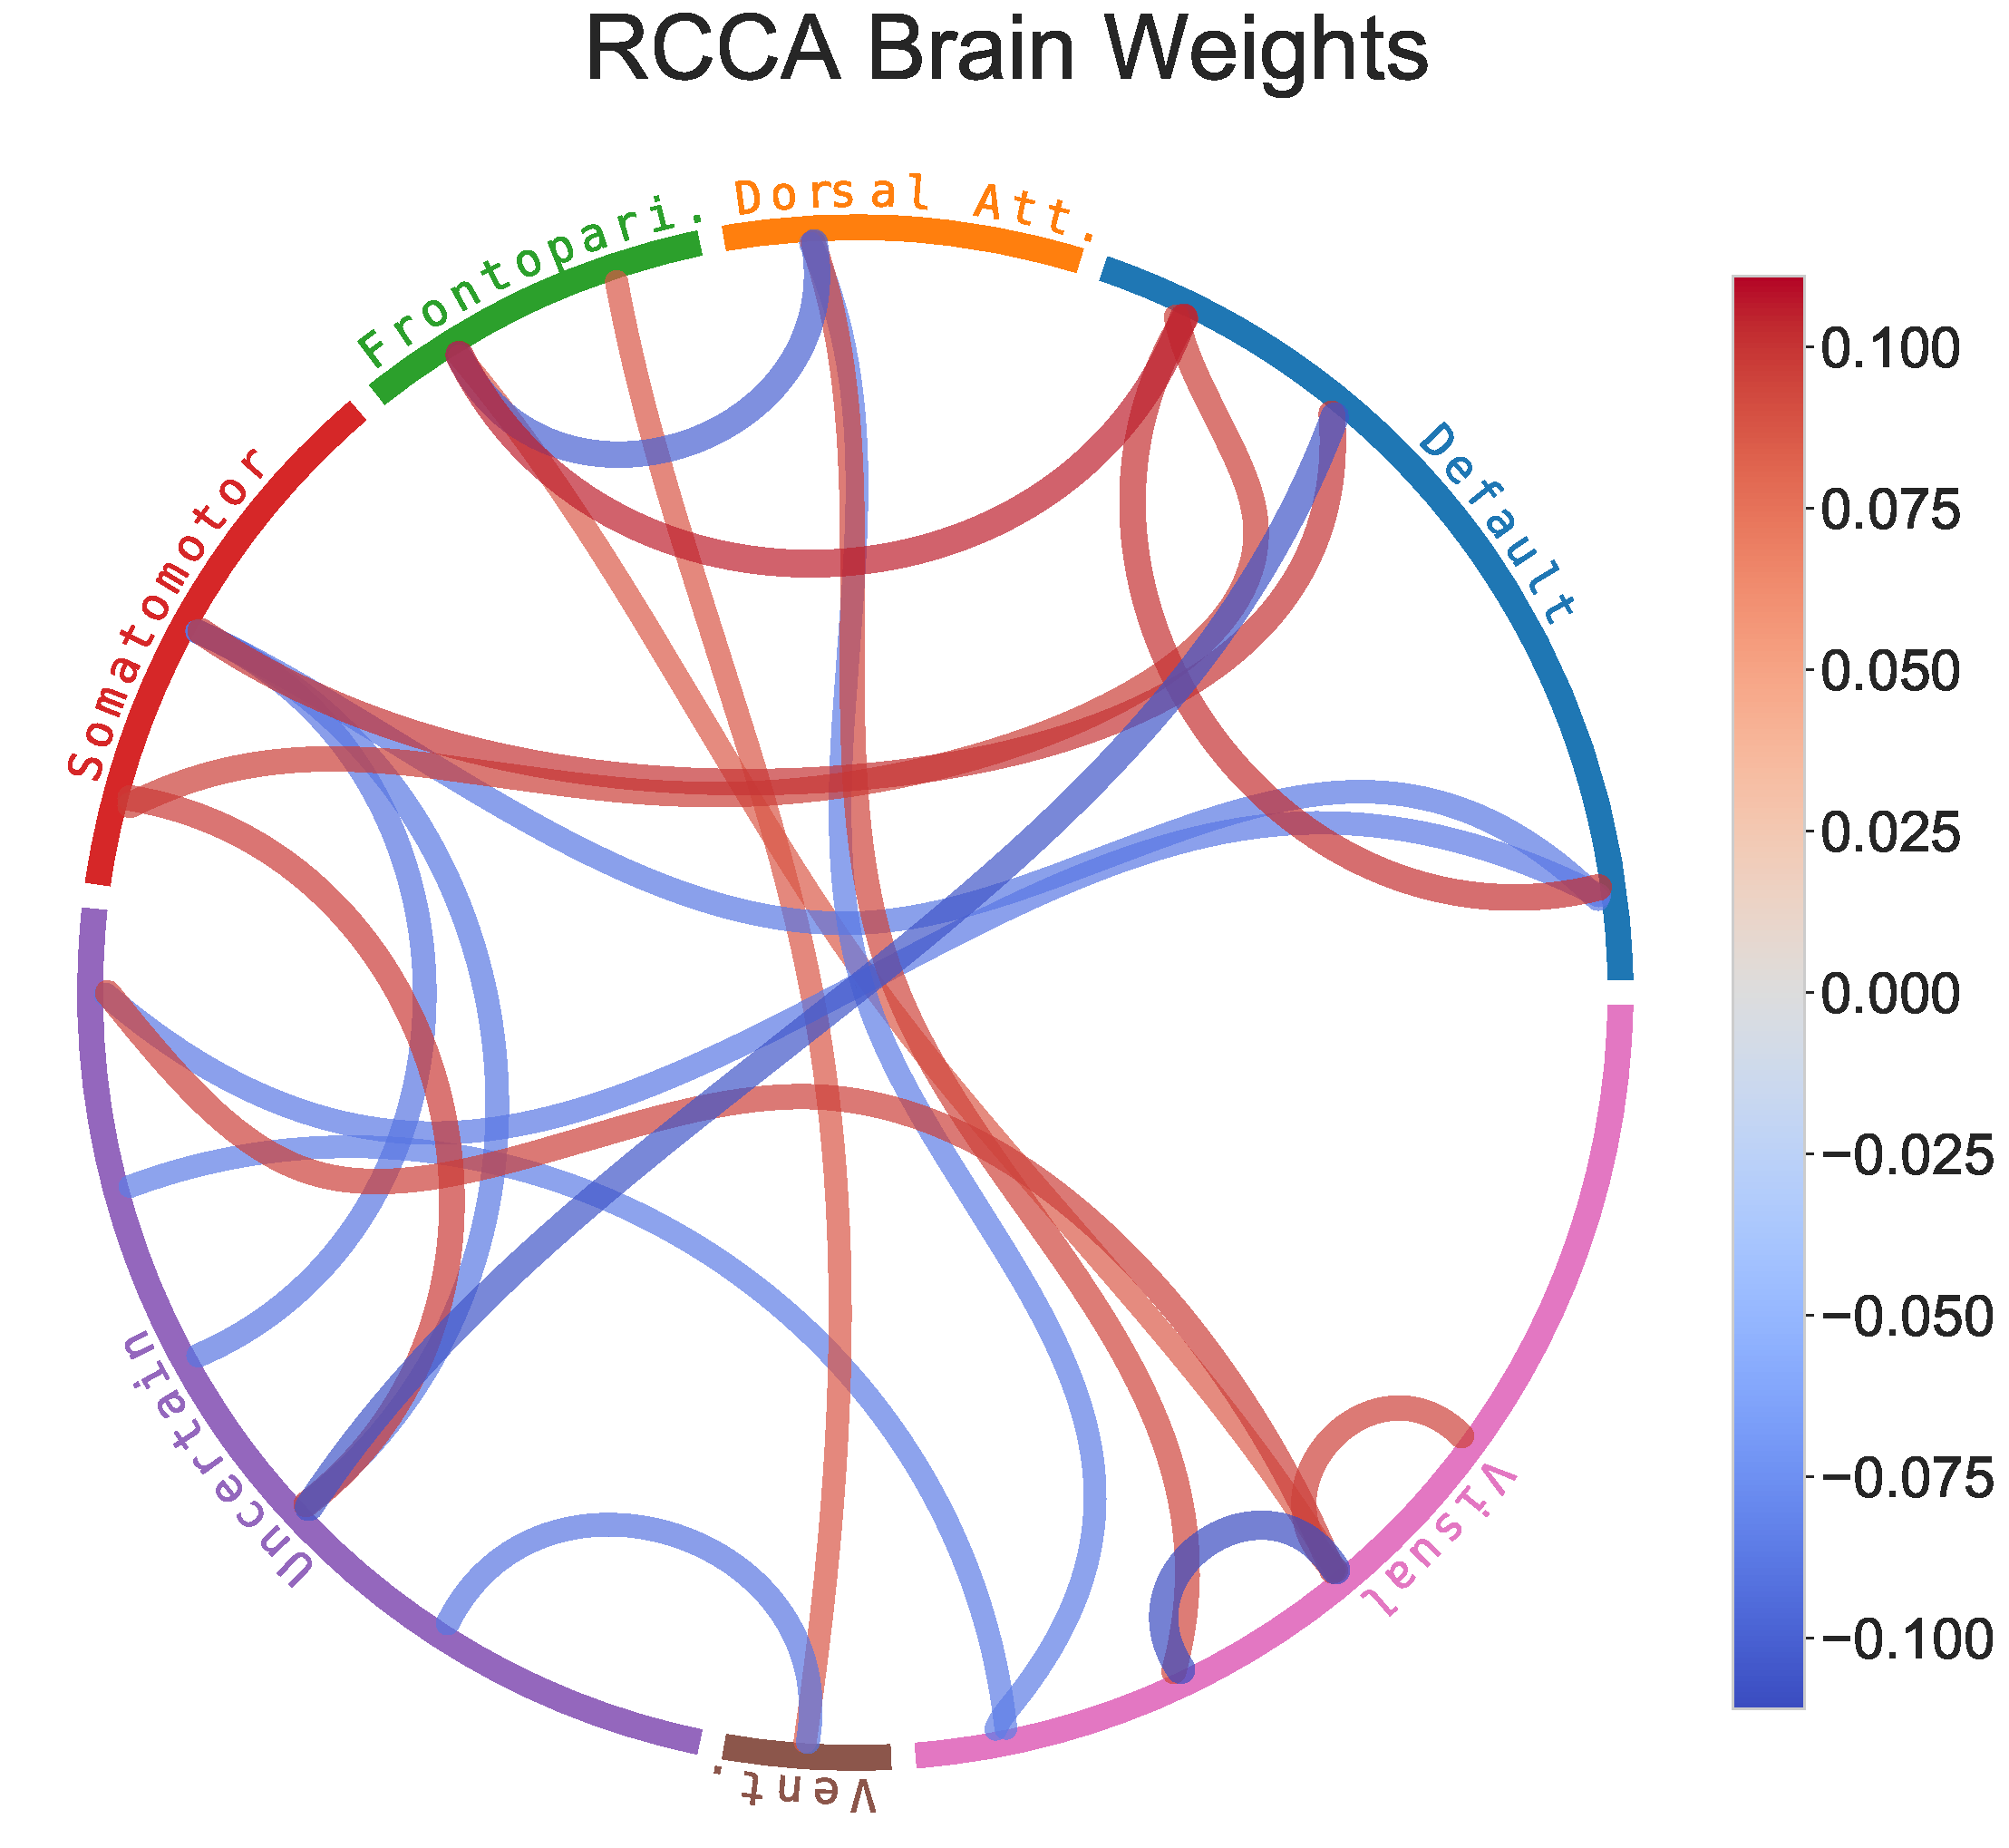
\includegraphics[width=0.49\linewidth]{figures/hcp/RCCA brain weights}
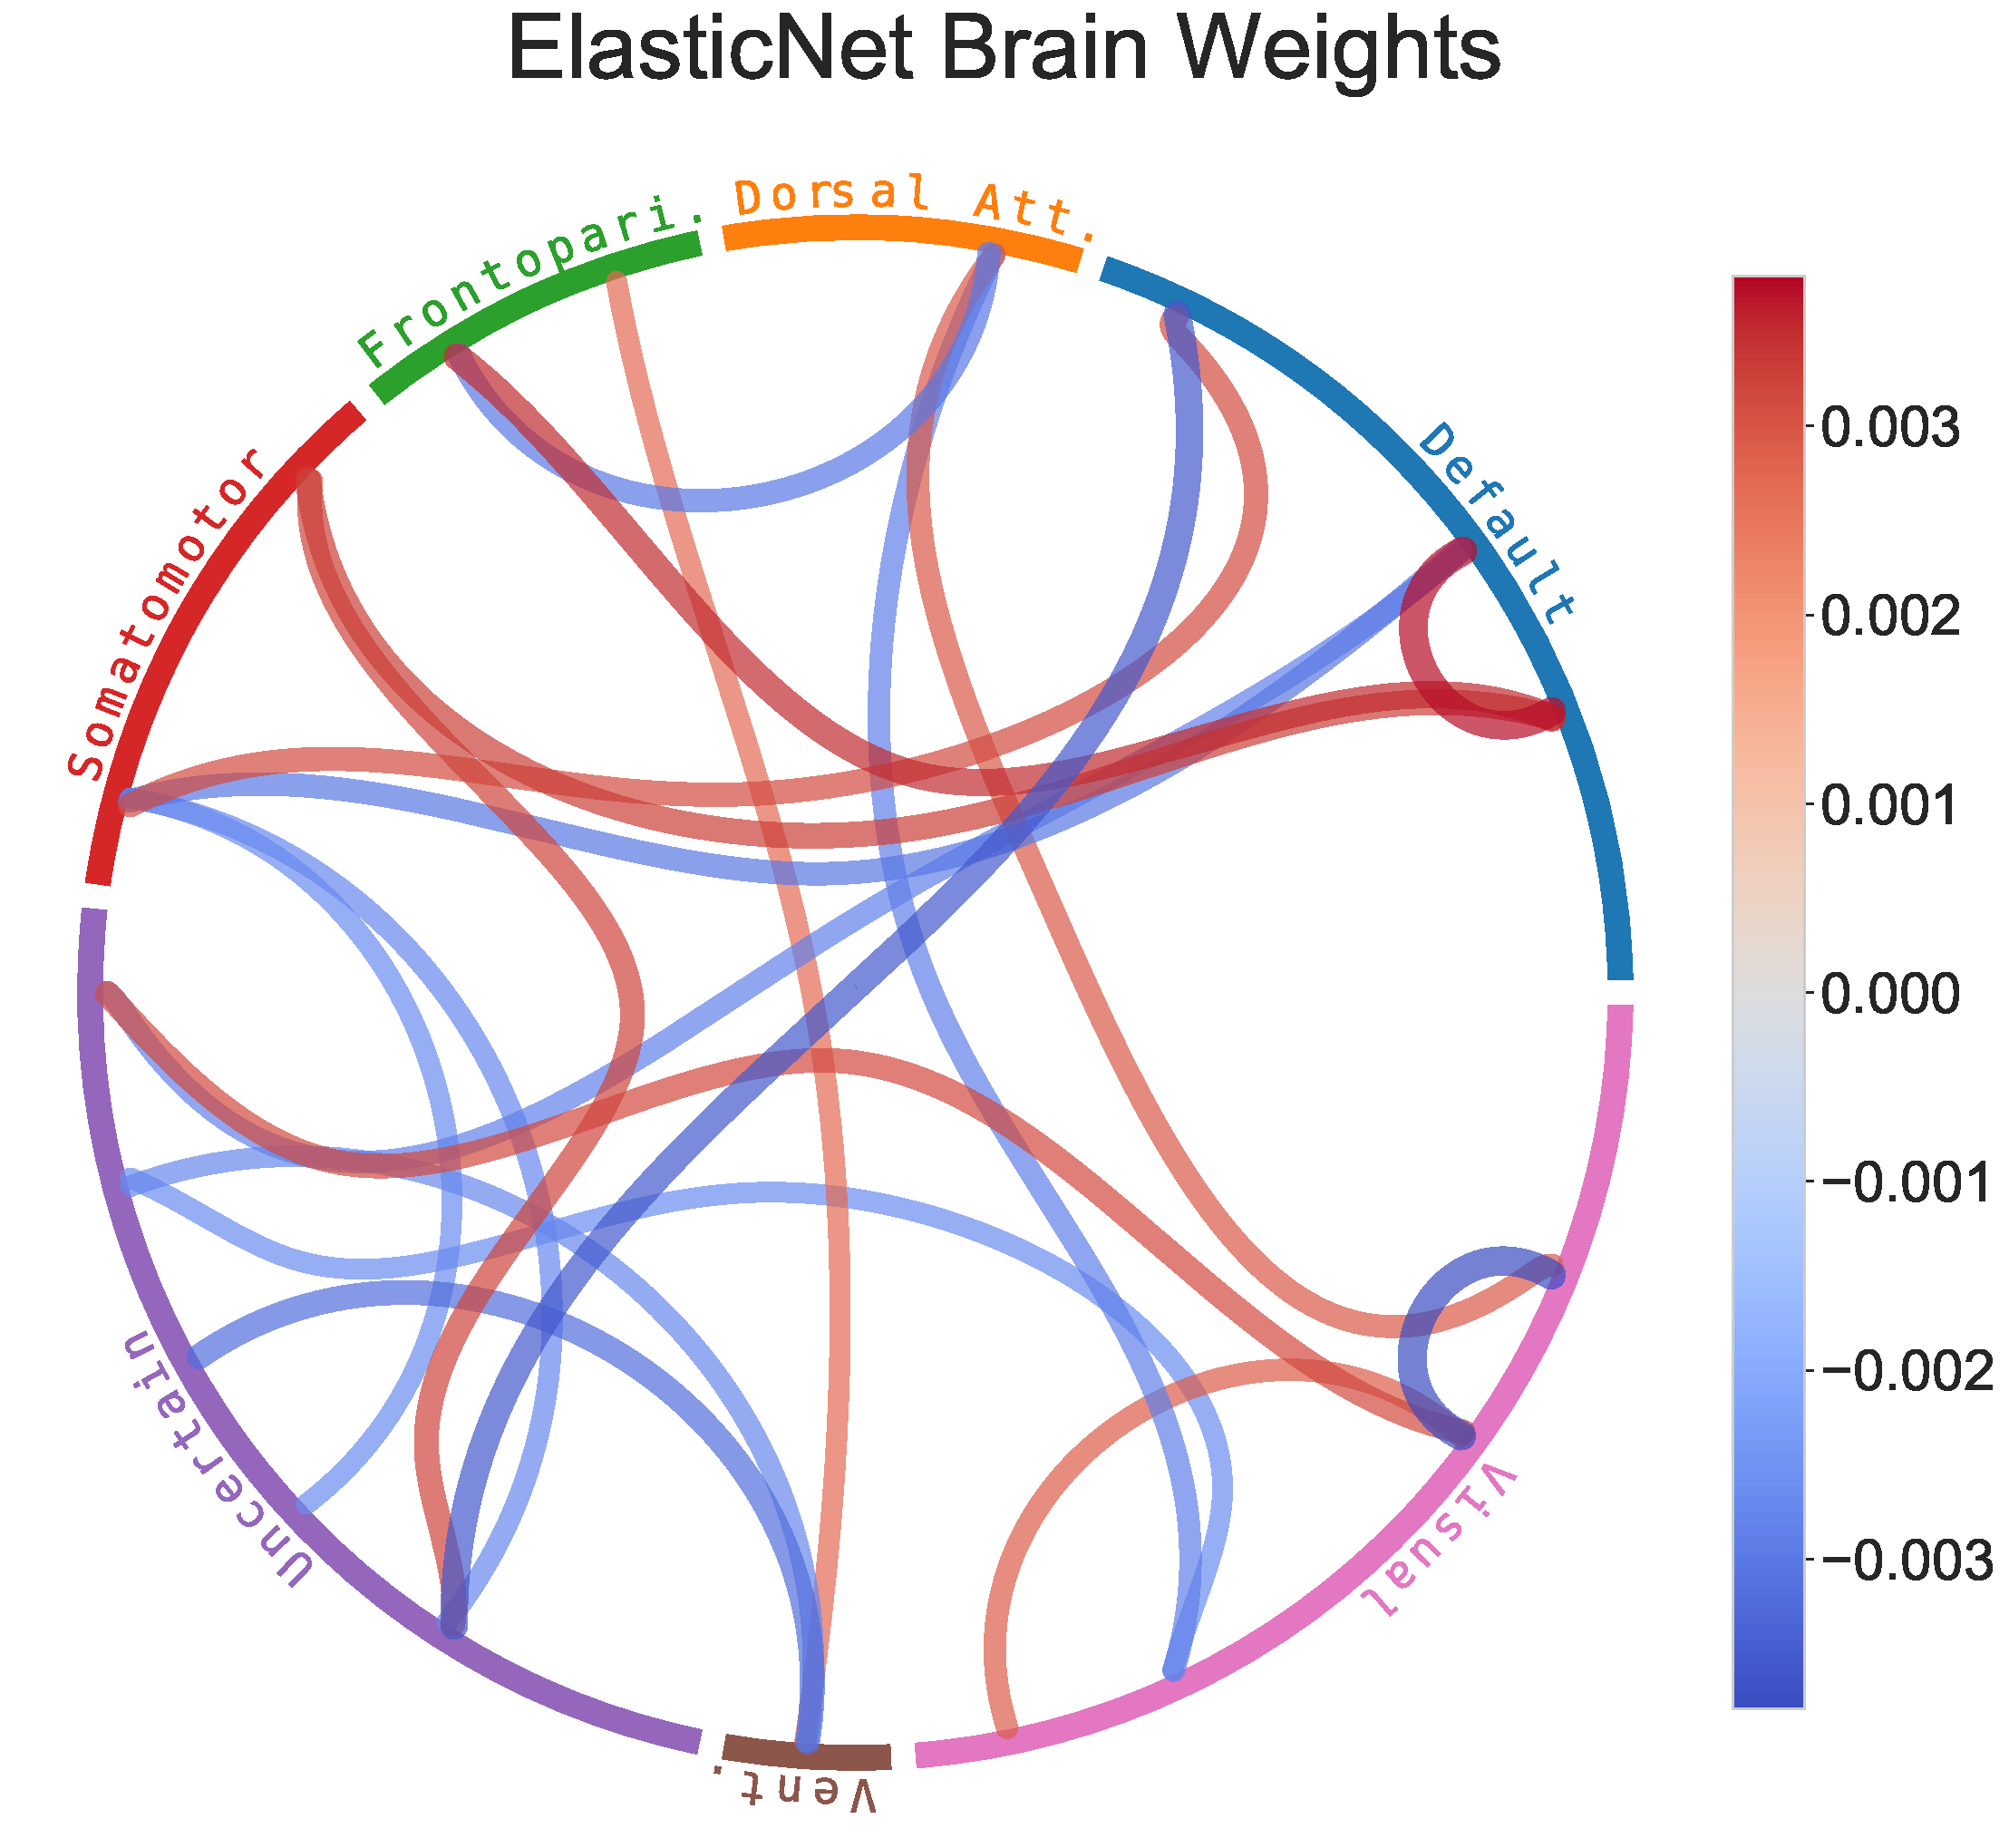
\includegraphics[width=0.49\linewidth]{figures/hcp/ElasticNet brain weights}
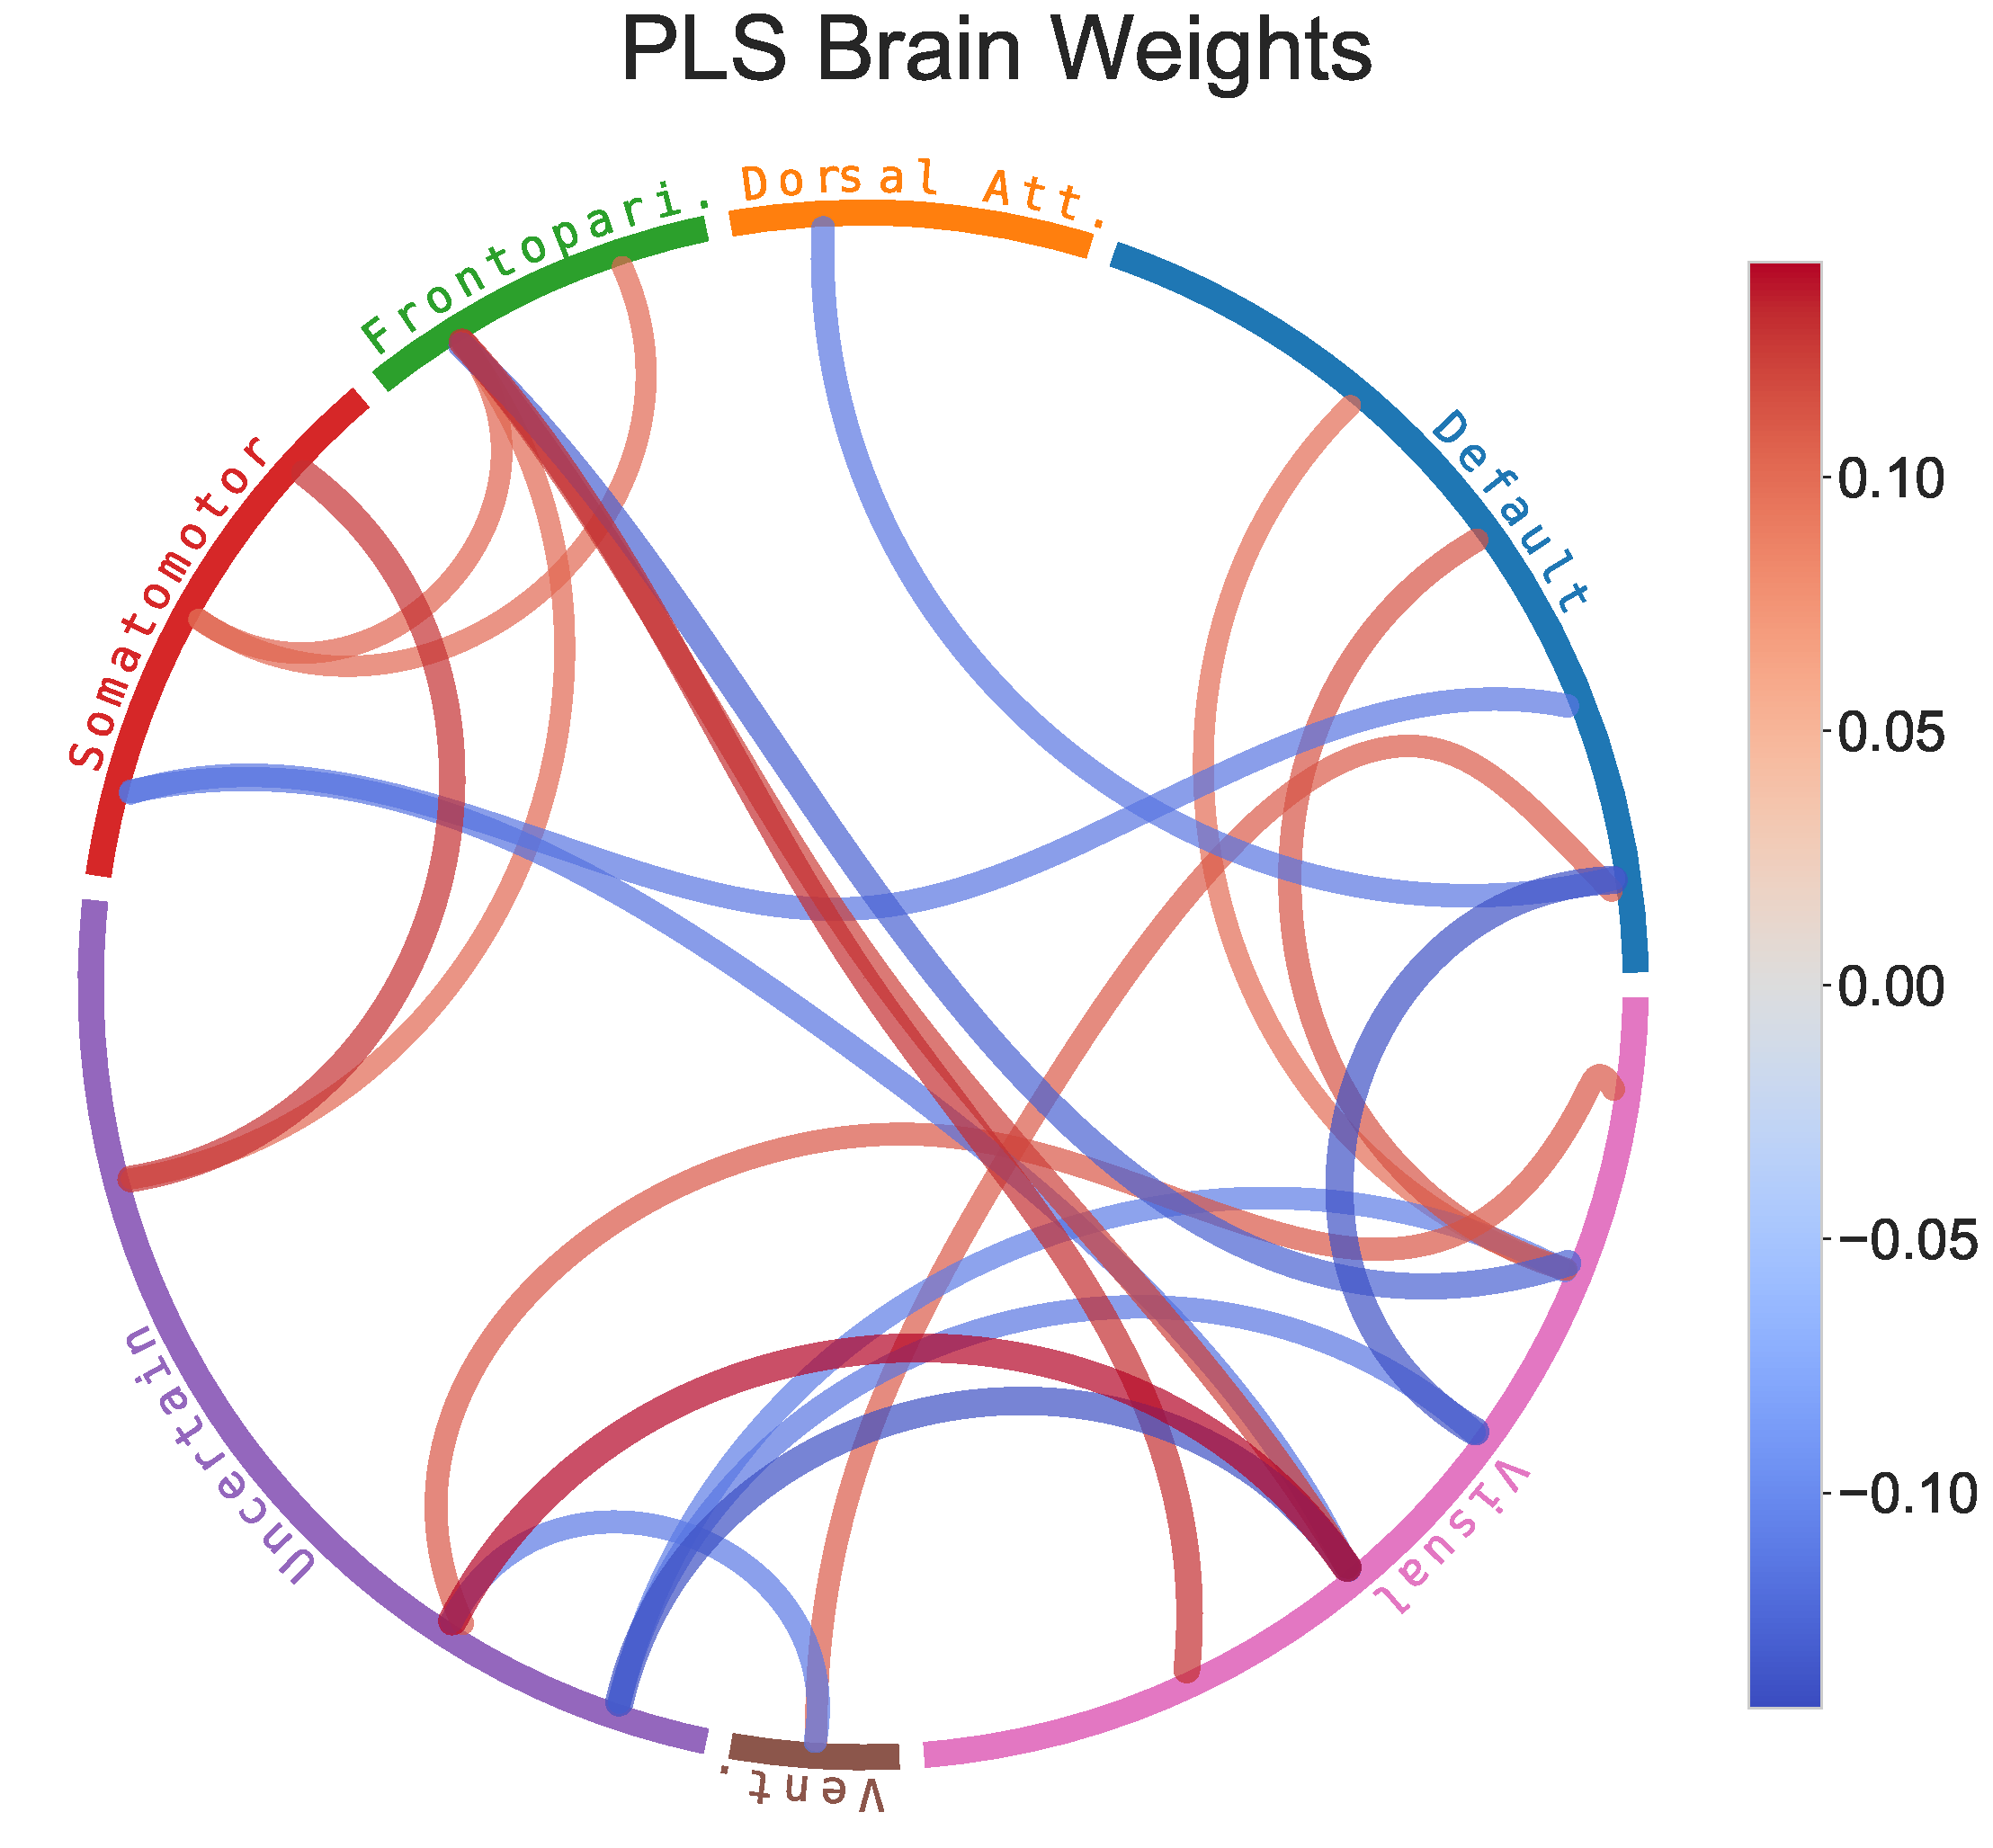
\includegraphics[width=0.49\linewidth]{figures/hcp/PLS brain weights}
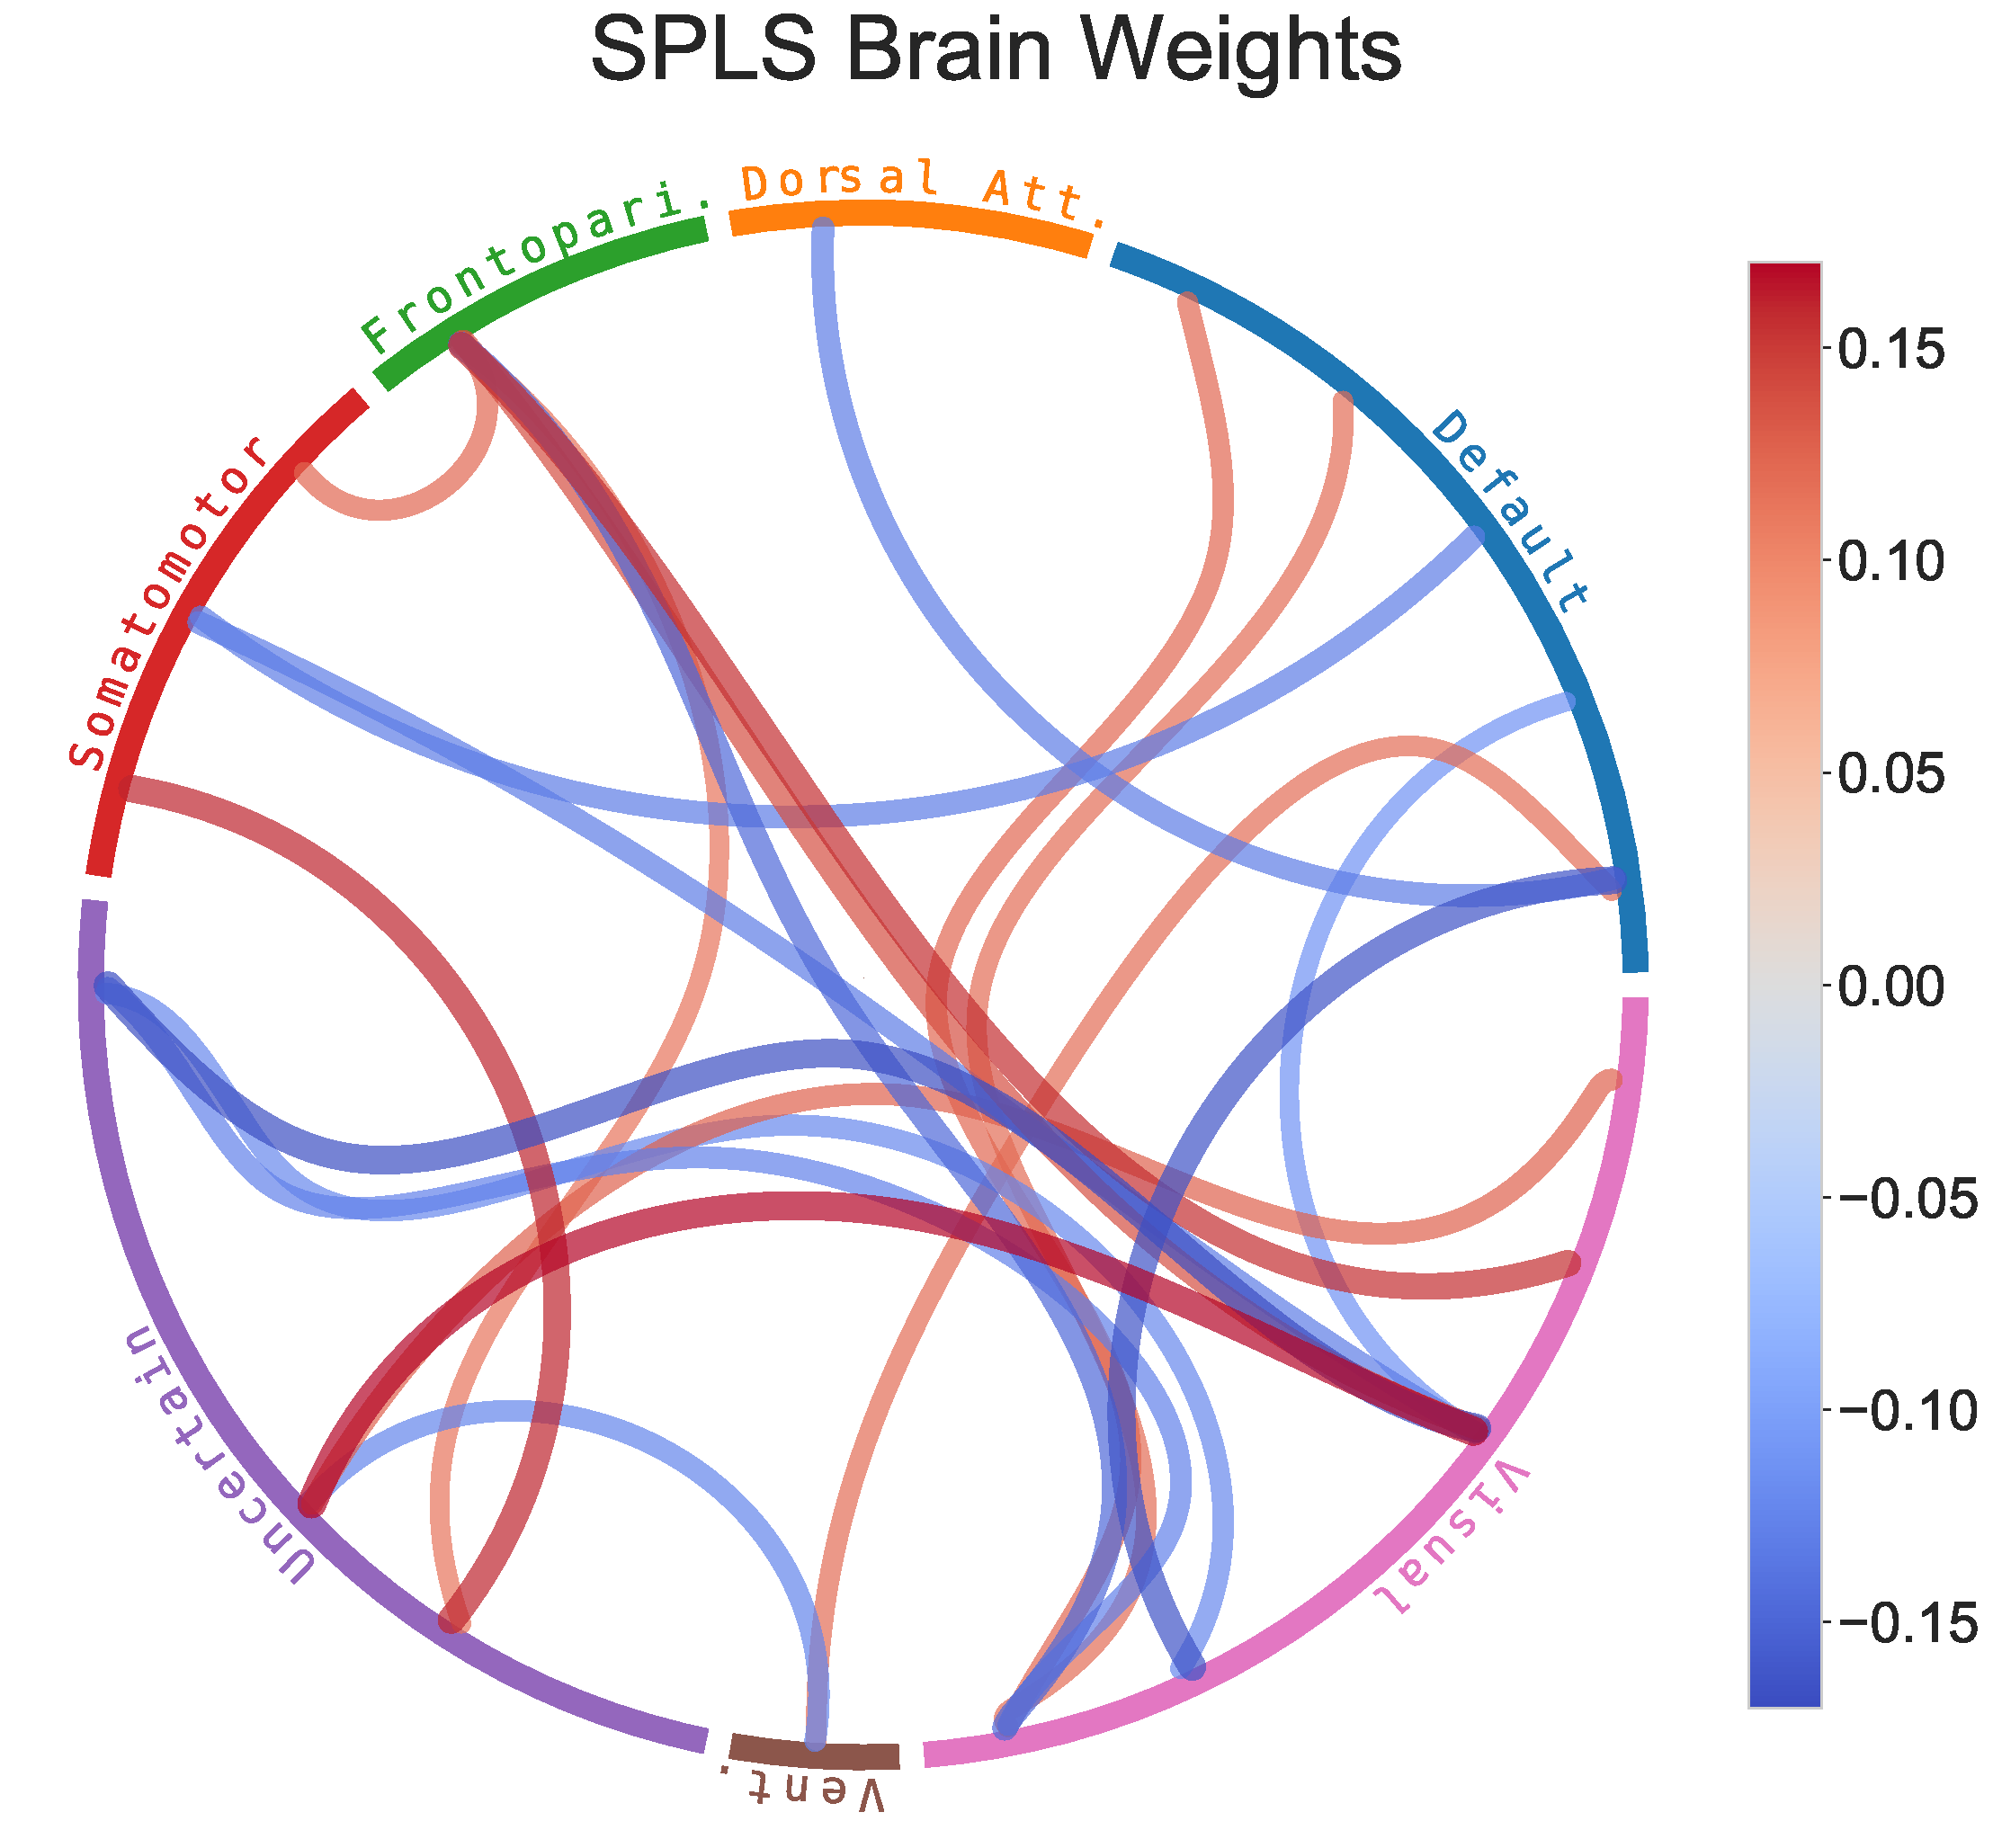
\includegraphics[width=0.49\linewidth]{figures/hcp/SPLS brain weights}
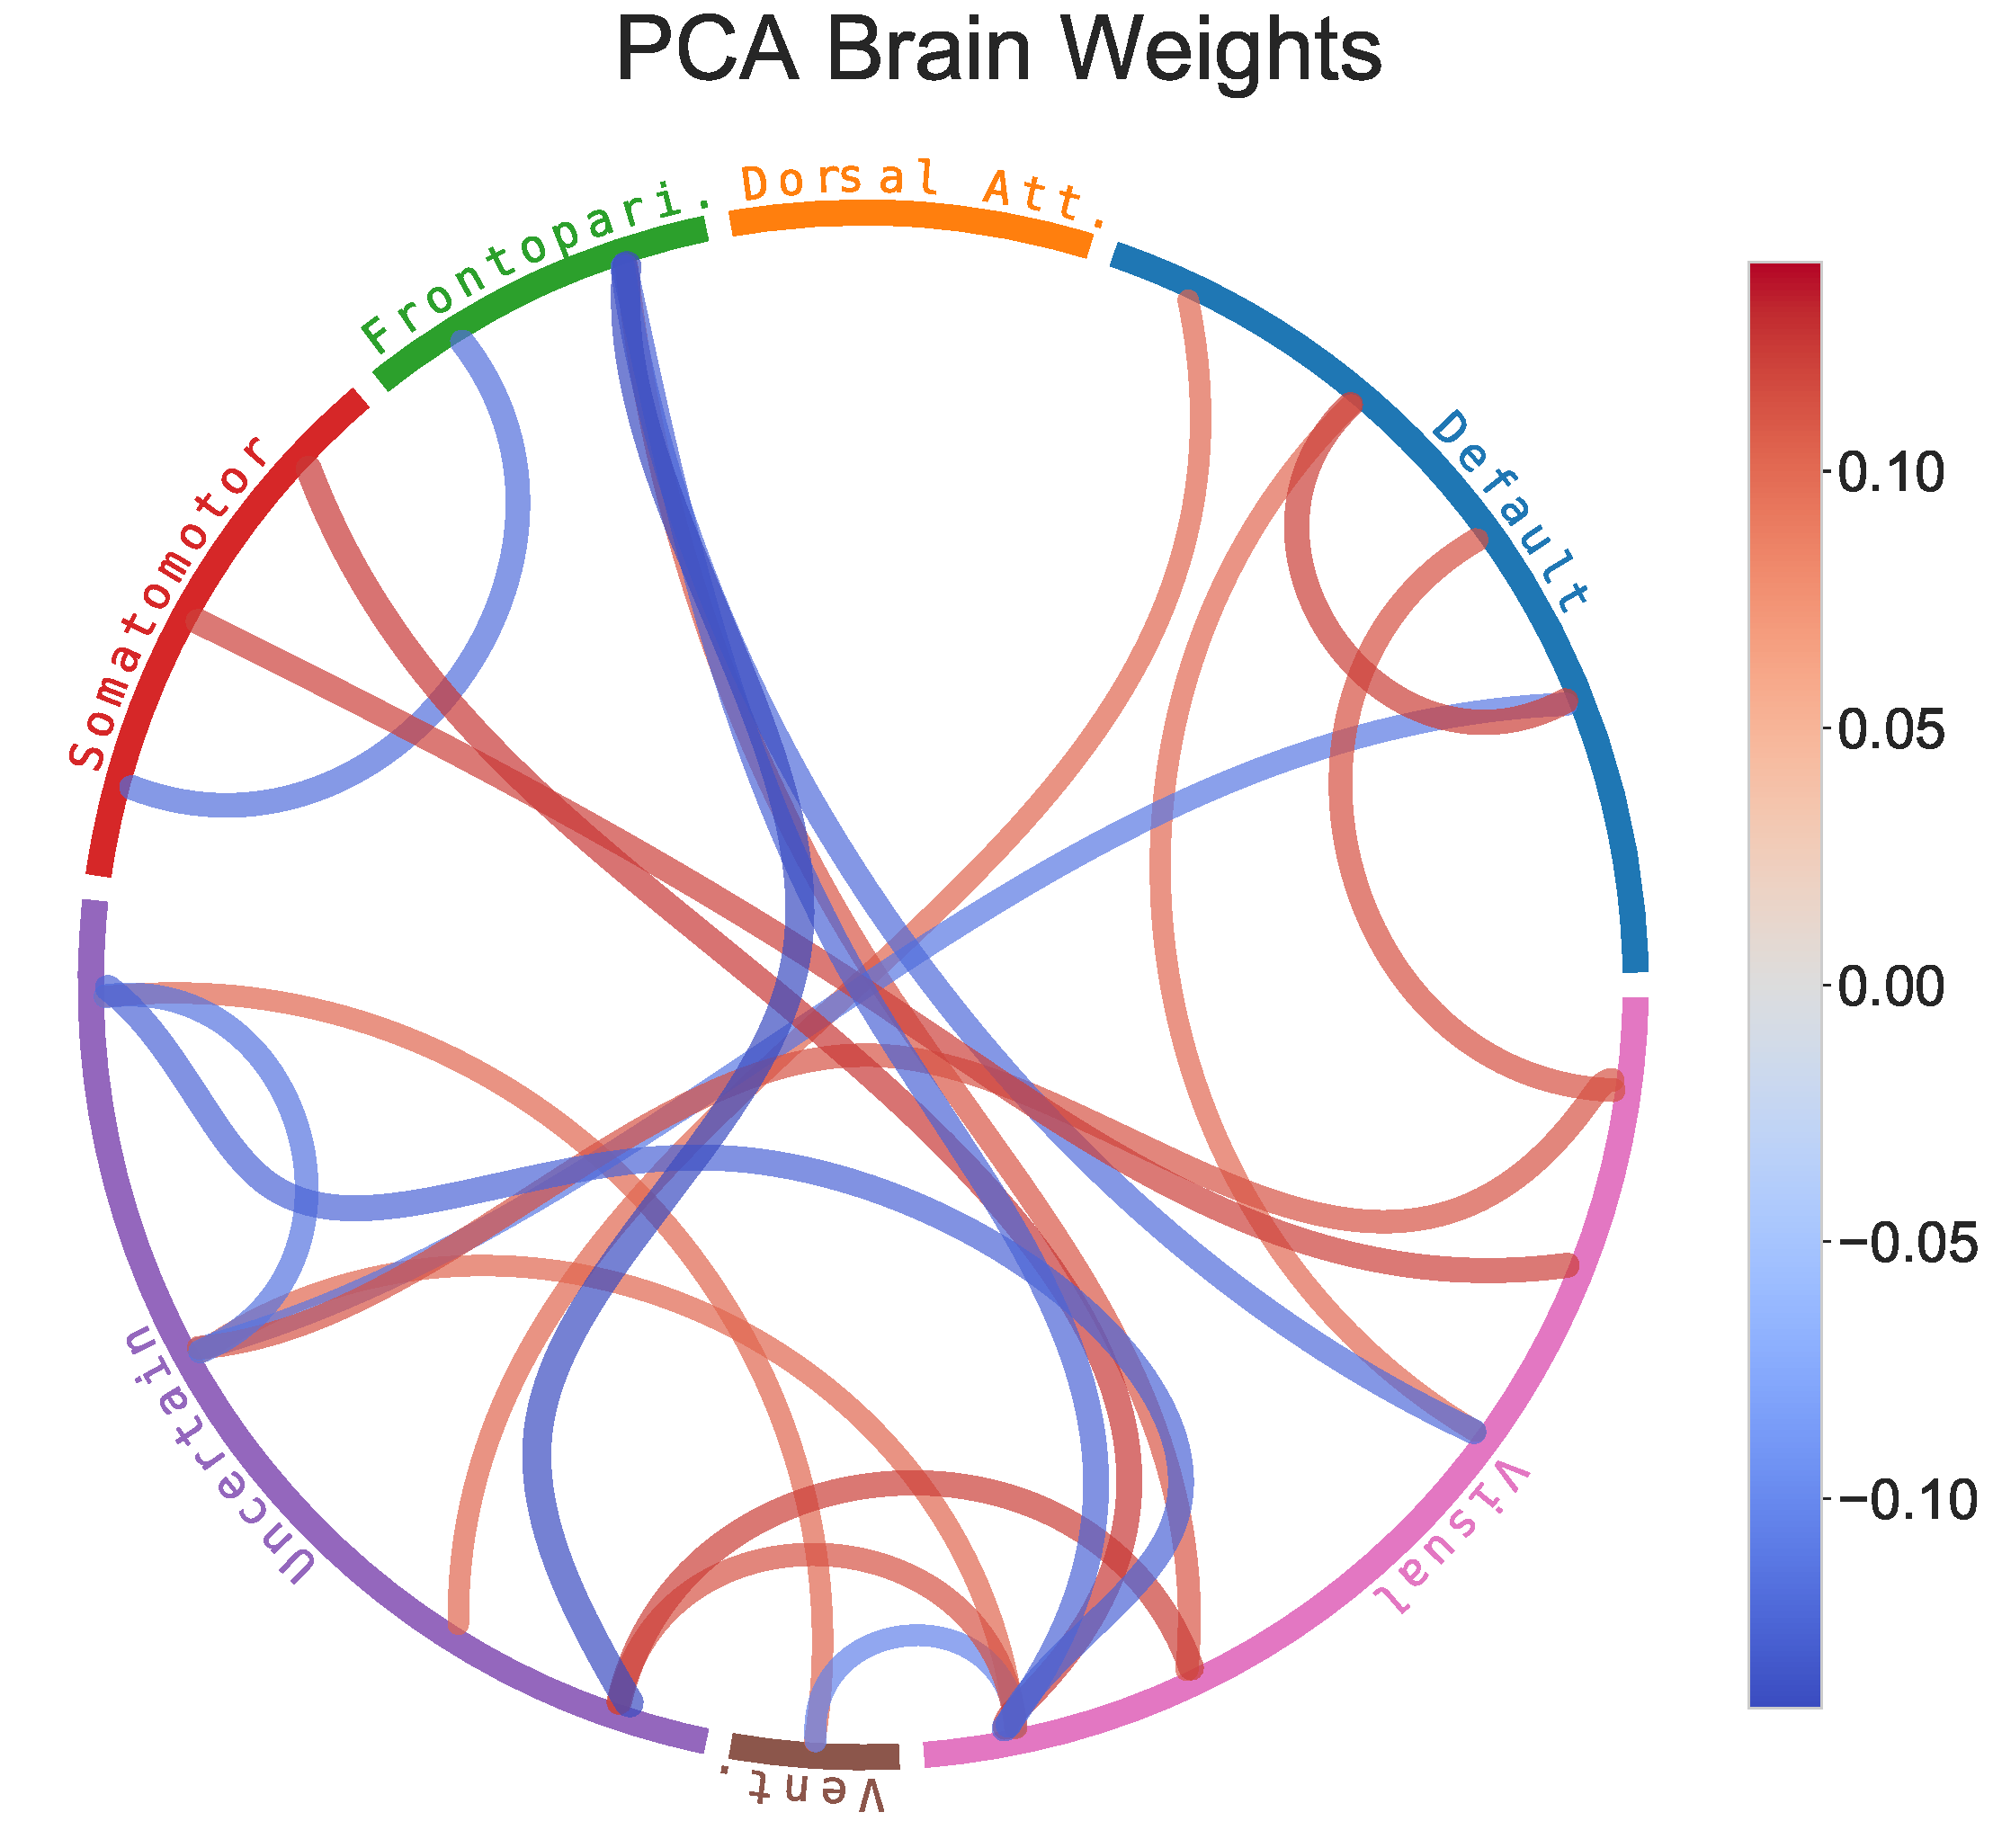
\includegraphics[width=0.49\linewidth]{figures/hcp/PCA brain weights}
\caption{Chord diagrams of the top 8 positive and negative brain \gls{weights} for each model.}\label{fig:chord_weights}
\end{figure}

%\paragraph{Surface Map Parcellations}
%The brain surface plots in Figure~\ref{fig:brain} represent maps of brain connection strength increases/decreases, which
%were obtained by weighting each node’s parcel map with the GFA edge-strengths summed across the edges
%connected to the node.
%In Figure~\ref{fig:brain}, we show increases on the left and decreases on the right.
%
%\textcolor{red} Need to find something biologically useful to say about these.
%
%\begin{figure}
%\centering
%\includegraphics[width=\linewidth]{figures/hcp/PCA brain weights surface}
%\includegraphics[width=\linewidth]{figures/hcp/RCCA brain weights surface}
%\includegraphics[width=\linewidth]{figures/hcp/ElasticNet brain weights surface}
%\includegraphics[width=\linewidth]{figures/hcp/PLS brain weights surface}
%\includegraphics[width=\linewidth]{figures/hcp/SPLS brain weights surface}
%\caption{Map of CCA connection strength variations, with each node’s parcel map weighted by CCA edge-strength changes across edges involving that node.}\label{fig:brain}
%\end{figure}

\subsubsection{Sparsity of Weights}

Table \ref{tab:brain-behaviour-weights-hcp} shows the number of non-zero \gls{weights} for each model.
We can see that tuned SPLS and Elastic Net do find sparse weights, but given the minimal difference in performance, it is not convincing evidence that this is a useful property.

\begin{table}[h]
\centering
\caption{Number of non-zero \gls{weights} for each model.}
\begin{tabular}{|c|c|c|}
\hline
Model &  Brain Weights &  Behaviour Weights \\
\hline
PCA & 300 & 145 \\
RCCA & 300 & 145 \\
Elastic Net & 241 & 96 \\
PLS & 300 & 145 \\
SPLS & 118 & 56 \\
\hline
\end{tabular}\label{tab:brain-behaviour-weights-hcp}
\end{table}

\newpage
\subsection{Alzheimers Disease Neuroimaging Initiative (ADNI) Data}\label{subsec:adni}

We now turn to the ADNI data where our analysis is similar but visualized differently.
This is because the ADNI data contains structural MRI data rather than functional MRI data.

\subsubsection{Out of Sample Correlation}

In this experiment, the Elastic Net model outperformed all other models in terms of out-of-sample correlation (Figure~\ref{fig:performance}).
The RCCA model also outperformed the PLS and SPLS models while SPLS outperformed PLS.
Suprisingly, PCA performed almost as well as PLS.

\begin{figure}
\centering
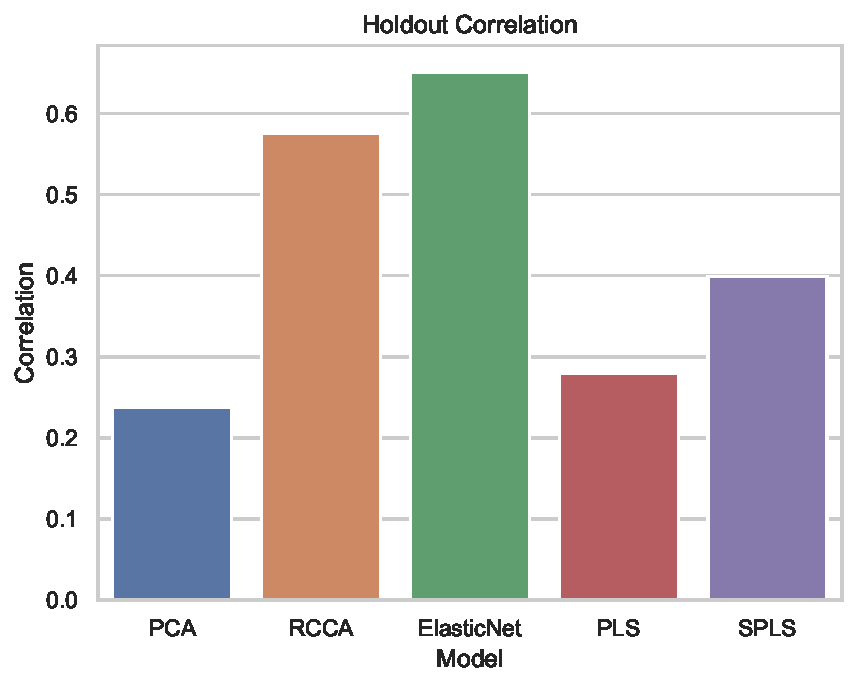
\includegraphics[width=0.5\linewidth]{figures/adni/holdout_correlations}
\caption{Out-of-sample canonical correlations for each model.}\label{fig:performance}
\end{figure}

\subsubsection{Behaviour Weights}

As for the HCP data, Figure \ref{fig:adni-beh} plots the top 8 positive and negative non-imaging \gls{weights} for each model.
Some of the identified behavioural \gls{weights} including a number of orientation tests are similar across all of the models, including even PCA.
This is indicative of the strong shared signal between the behavioural data and the brain structure data.
SPLS and Elastic Net both hone in on the orientation and recall tests in the weight space.
The RCCA and Elastic Net models are suprisingly different in the weight space, with the RCCA \gls{weights} on a couple of attention and calculation tests in addition to the ubiquitous orientation and recall tests.

\begin{figure}
\centering
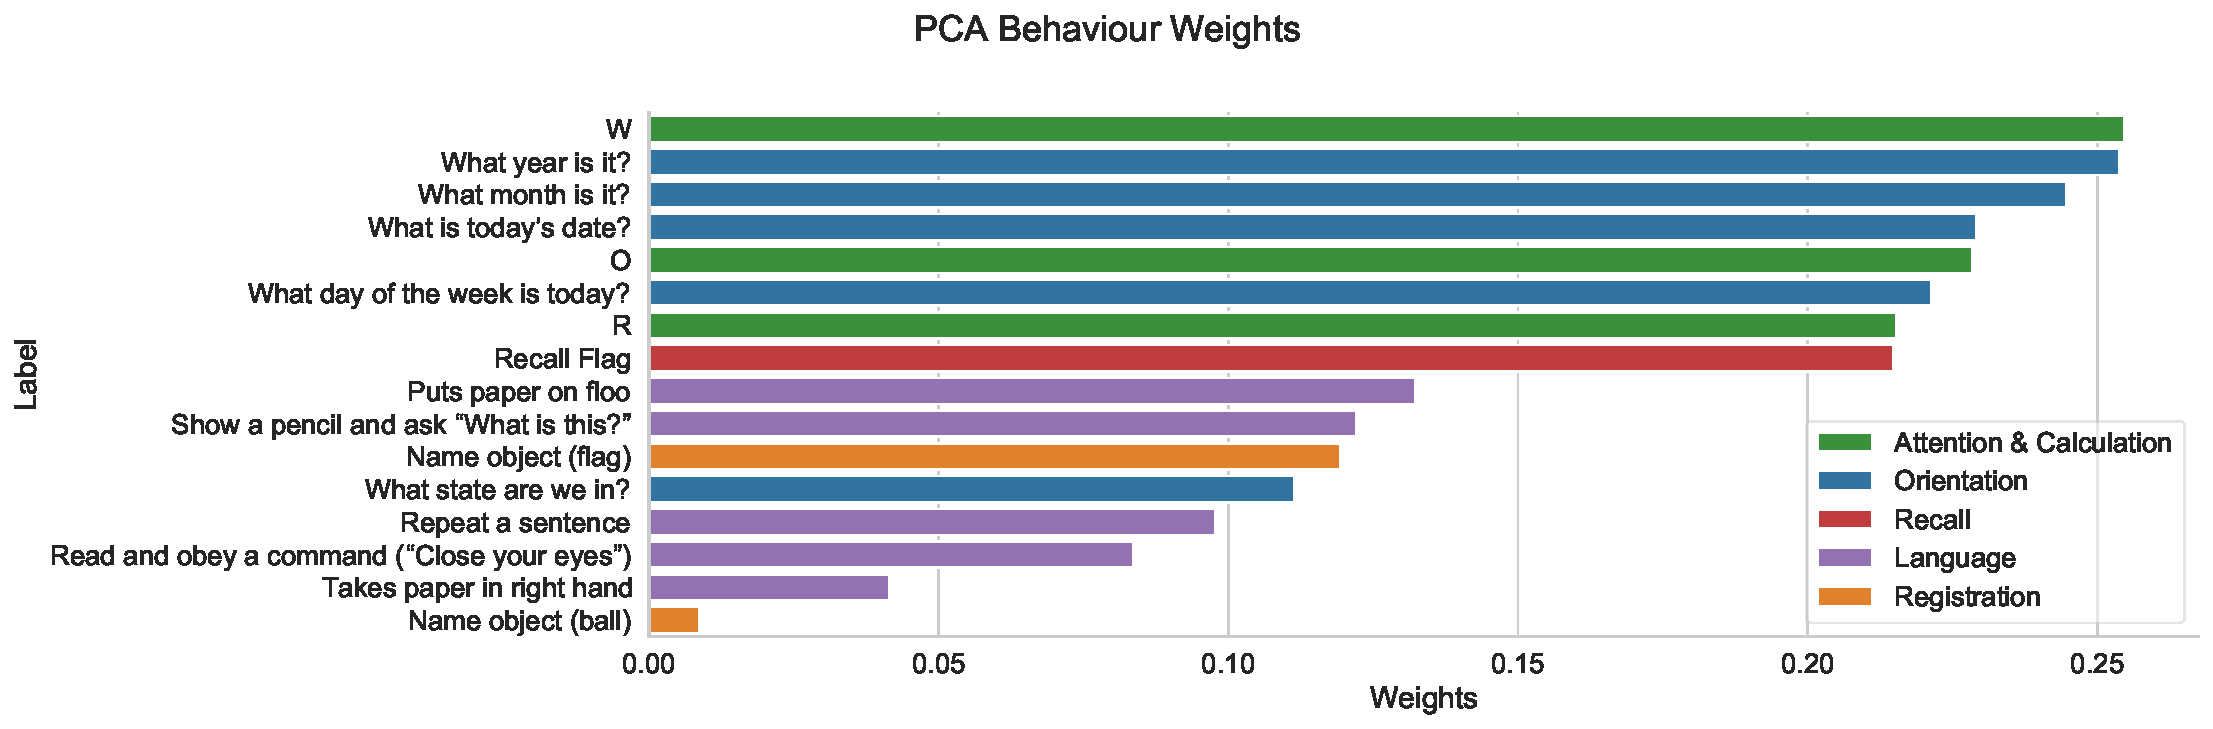
\includegraphics[width=0.8\linewidth]{figures/adni/PCA behaviour weights}
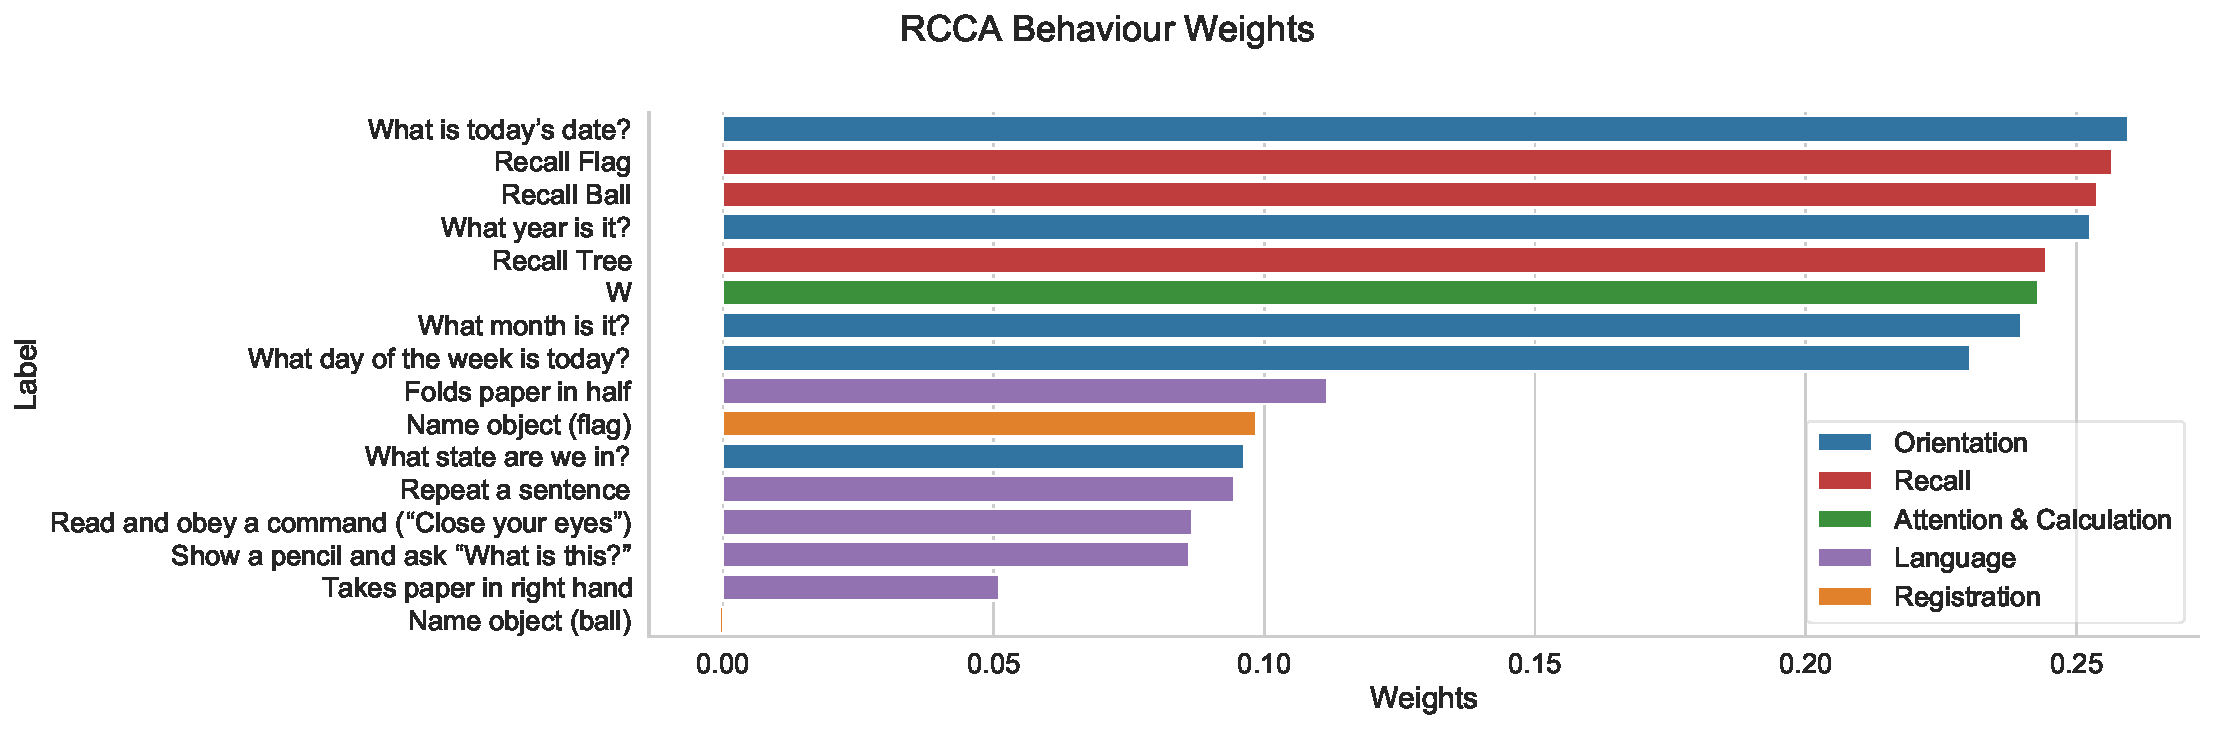
\includegraphics[width=0.8\linewidth]{figures/adni/RCCA behaviour weights}
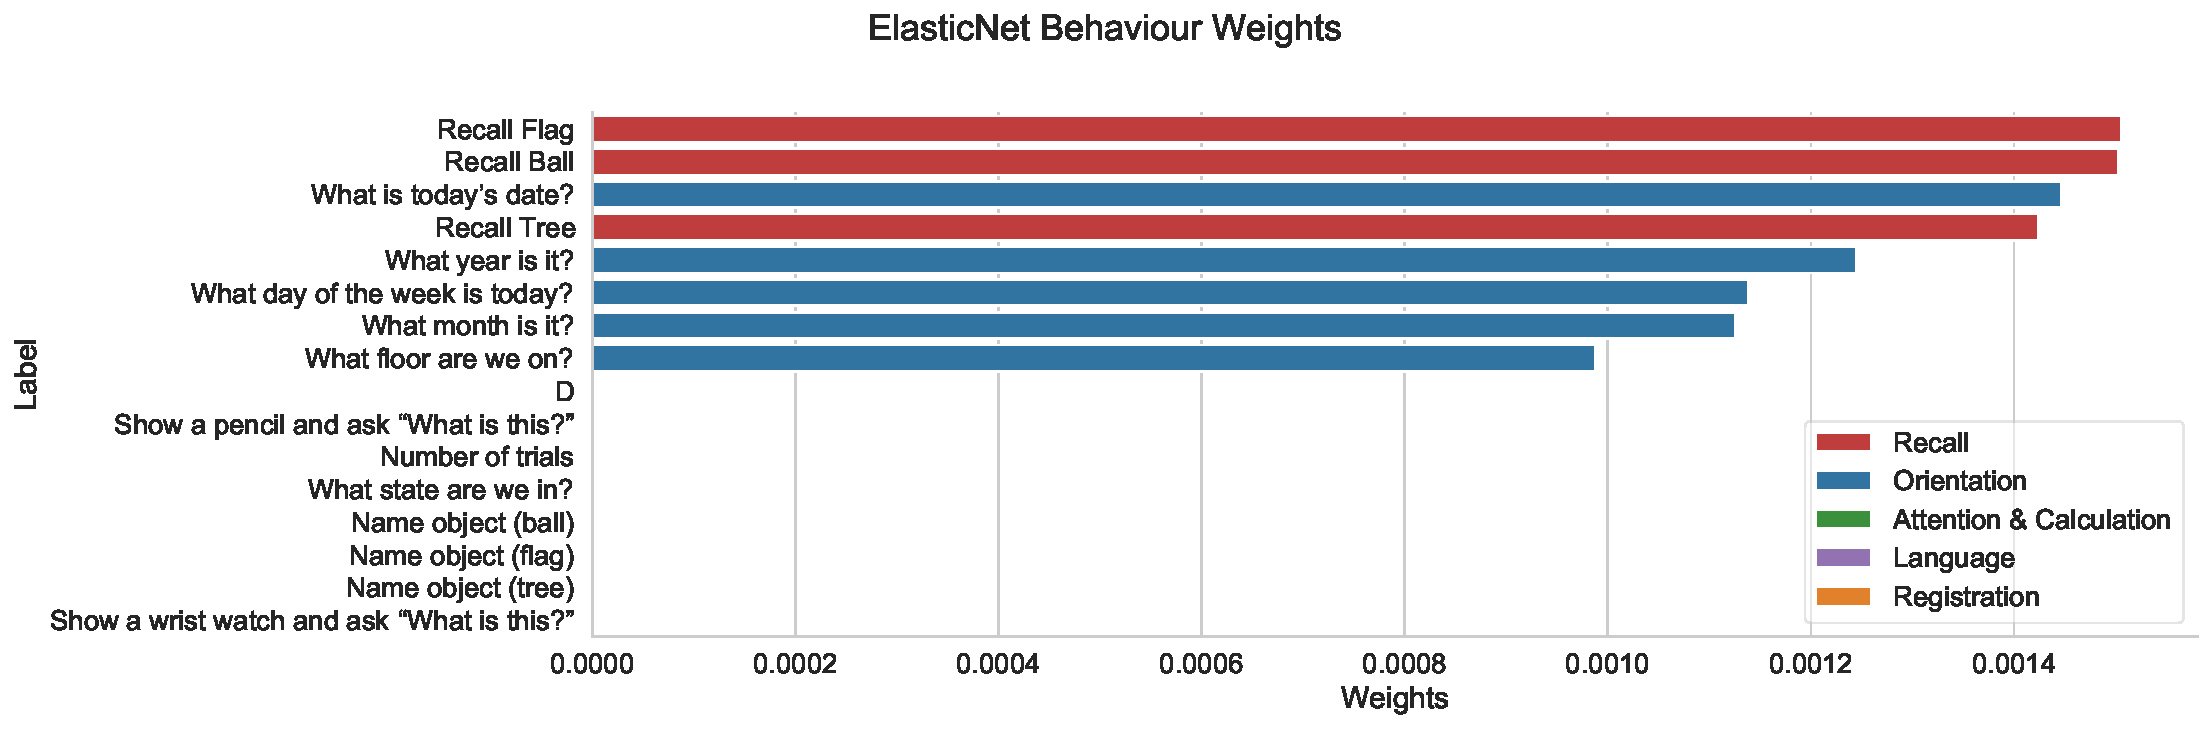
\includegraphics[width=0.8\linewidth]{figures/adni/ElasticNet behaviour weights}
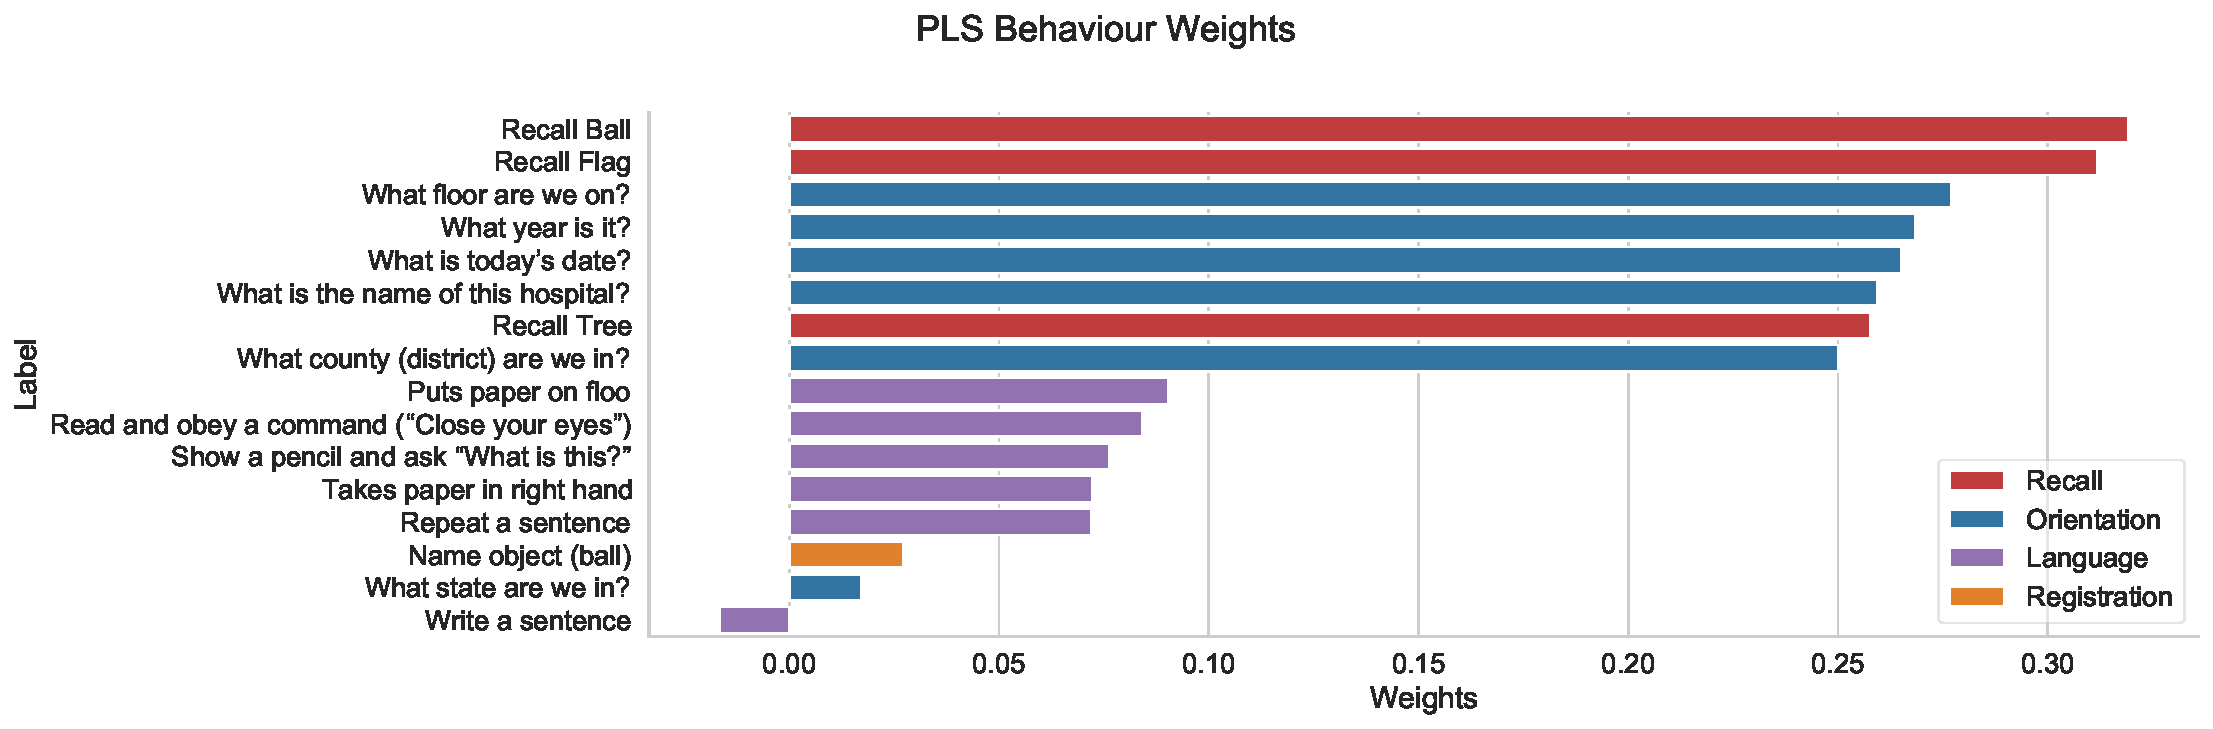
\includegraphics[width=0.8\linewidth]{figures/adni/PLS behaviour weights}
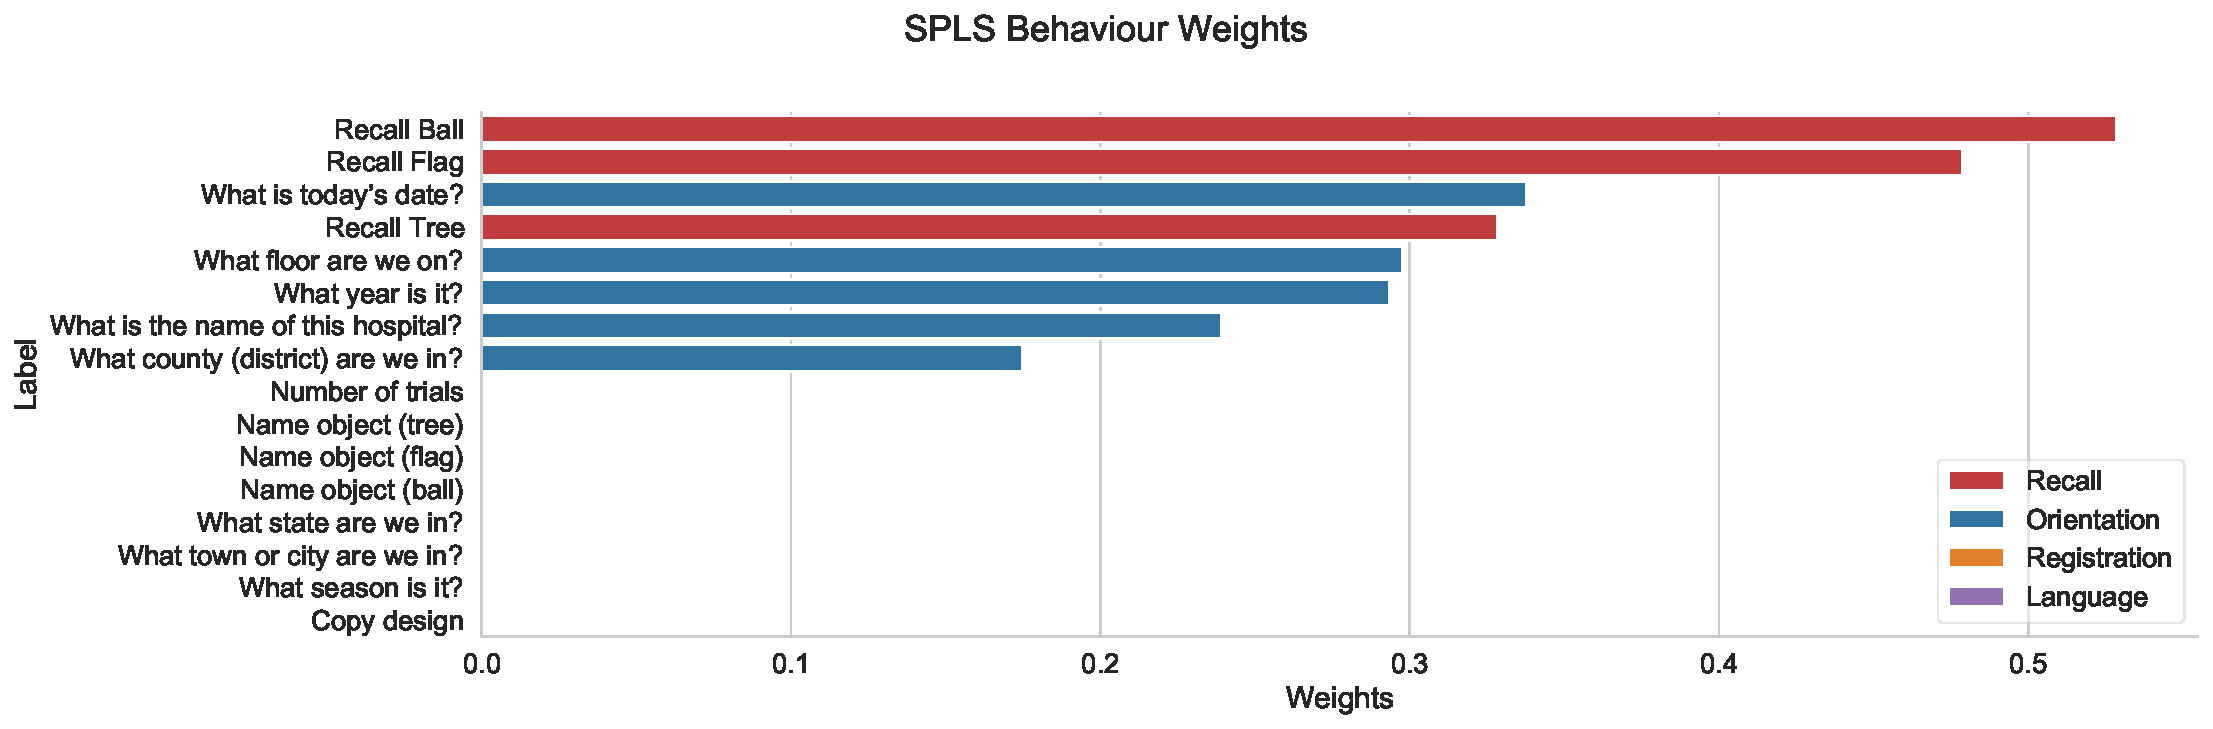
\includegraphics[width=0.8\linewidth]{figures/adni/SPLS behaviour weights}
\caption{Bar plots of the behaviour \gls{weights} for each model.}\label{fig:adni-beh}
\end{figure}

\subsubsection{Brain Structure Weights}

We plot the \gls{weights} as a mosaic plot with 3 slices in each direction in Figure~\ref{fig:adni-brain}.
Previous work using SPLS with the ADNI dataset identified the same striking pattern of \gls{weights} with the model strikingly selecting the hippocampal weights\cite{monteiro2016multiple}.
The Elastic Net has a less visually appealing selection of weights, with a honeycomb pattern near the edges of the brain and likewise for RCCA.
It is noticeable that PCA, PLS and SPLS both \gls{weights} in the same direction whereas RCCA and Elastic Net weight different regions with opposite signs.

\begin{figure}
\centering
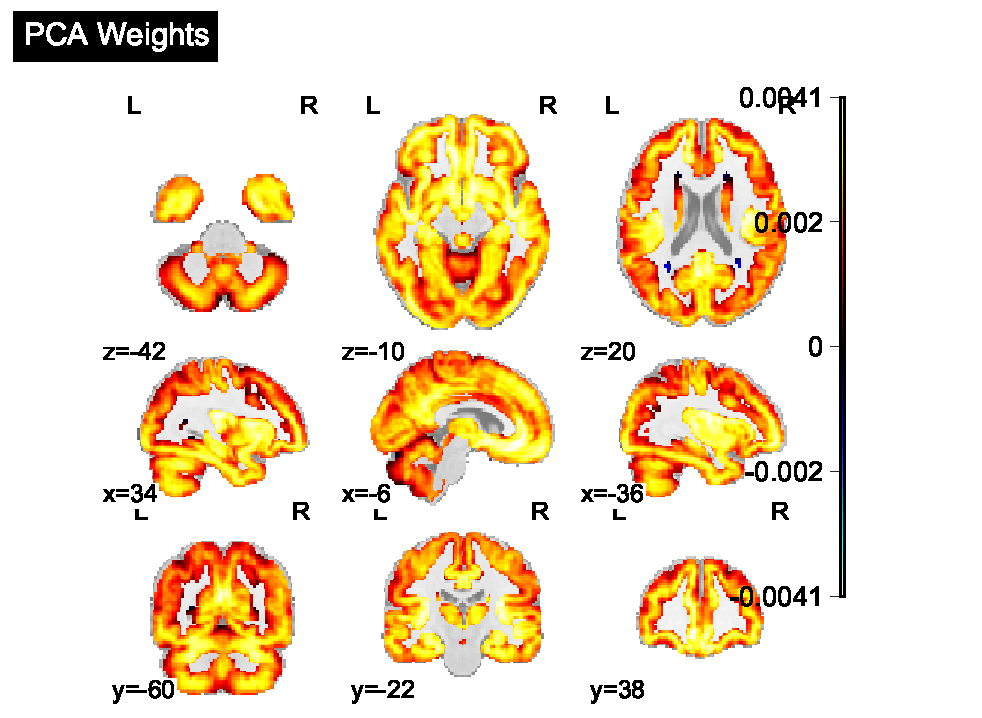
\includegraphics[width=0.45\linewidth]{figures/adni/PCA brain weights mosaic}
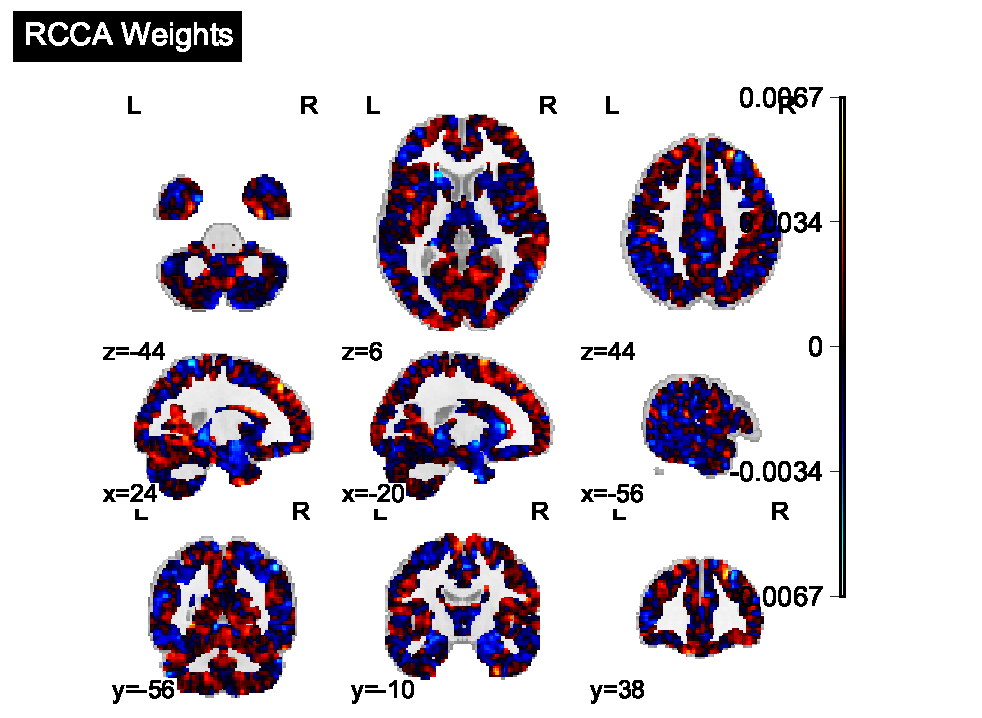
\includegraphics[width=0.45\linewidth]{figures/adni/RCCA brain weights mosaic}
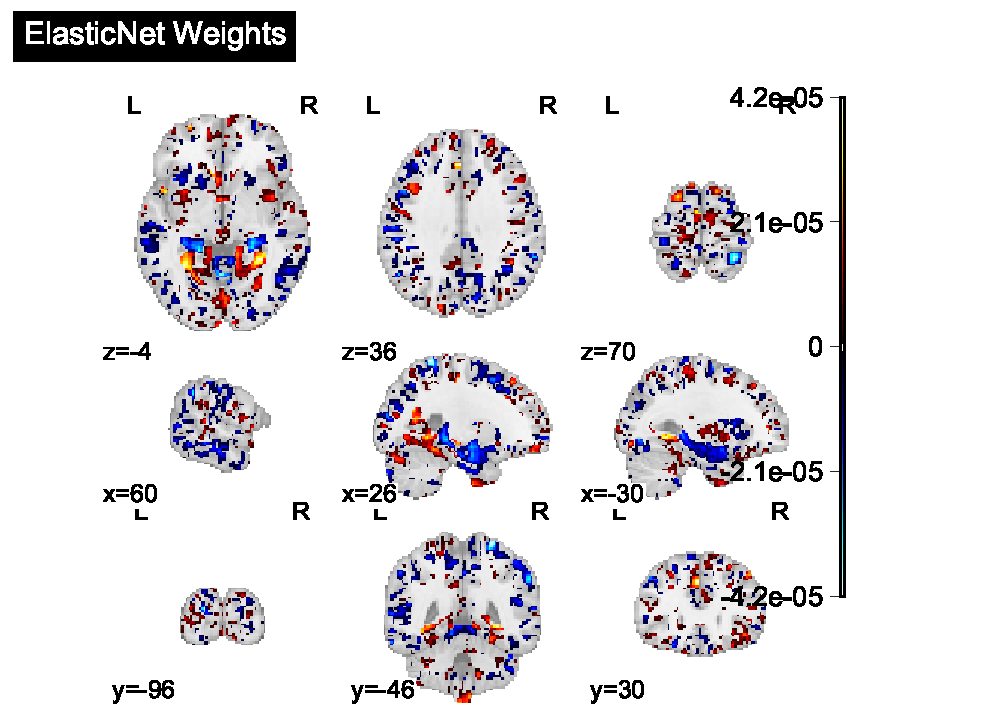
\includegraphics[width=0.45\linewidth]{figures/adni/ElasticNet brain weights mosaic}
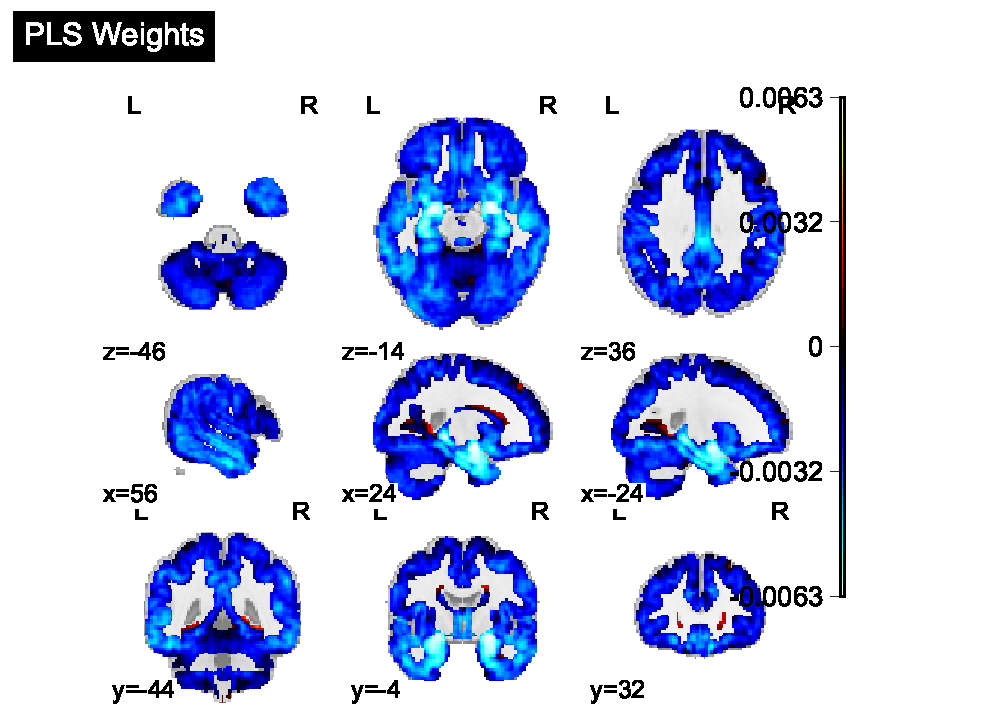
\includegraphics[width=0.45\linewidth]{figures/adni/PLS brain weights mosaic}
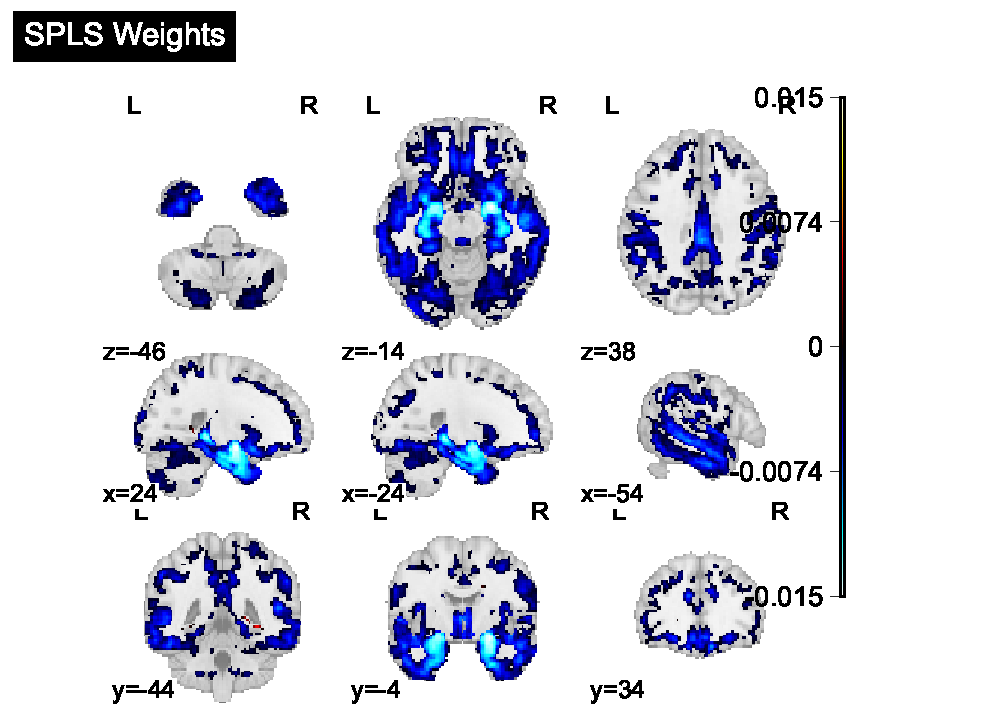
\includegraphics[width=0.45\linewidth]{figures/adni/SPLS brain weights mosaic}
\caption{Statistical maps of brain structure weights for each model.}
\end{figure}

\subsubsection{Sparsity of Weights}

Table~\ref{tab:brain-behaviour-weights-adni} once again shows the number of non-zero \gls{weights} for each model.
We can see that tuned SPLS and Elastic Net once again identify sparse weights.
In this case, the difference in performance is more convincing and suggests that this sparsity is less spuriously induced than for the HCP data.
This is supported by the fact that Elastic Net and SPLS models find a similar level of sparsity in the brain weights.
On the other hand SPLS finds a much sparser set of behavioural weights.

\begin{table}[h]
\centering
\caption{Number of non-zero \gls{weights} for each model.}
\begin{tabular}{|c|c|c|}
\hline
Model & Brain Weights & Behaviour Weights \\
\hline
PCA & 168130 & 31 \\
RCCA & 168130 & 31 \\
Elastic Net & 59617 & 17 \\
PLS & 168130 & 31 \\
SPLS & 74995 & 10 \\
\hline
\end{tabular}\label{tab:brain-behaviour-weights-adni}
\end{table}

\newpage
\newpage
\section{Discussion and Limitations}

In this section, we discuss the implications of our findings as well as the limitations of our study and the proposed FRALS method, some of which we address in later chapters of this thesis.

\subsection{Discussion}

\paragraph{Ridge CCA is typically much better than PLS across datasets:} Our results show that Ridge CCA is typically much better than PLS across datasets.
Much like regularised regression, it is unusual to need to use maximal ridge regularization even in high dimensions.
This means that while PLS might be more stable for a given dataset, it is not necessarily more stable across random samples from the same population.

\paragraph{FRALS is a useful tool for implementing Elastic Net CCA:} Our results show that FRALS is a useful tool for implementing Elastic Net CCA.

\subsection{FRALS Limitations}
While FRALS offers promising performance in terms of out-of-sample correlation, it does come with significant drawbacks, the most noteworthy being its computational inefficiency.
Below, we outline the primary factors contributing to the slow speed of FRALS and provide some insights into the computational bottlenecks.

\paragraph{Changing Regression Targets}\label{subsec:changing-regression-targets}
Adding to the computational burden is the fact that the regression targets, i.e., the projections of the other view, are not static but change dynamically throughout the algorithm's run.
Each update to the least squares solution consequently alters the global objective, leading to a constantly shifting landscape that the algorithm needs to navigate.
This also leads to a significant amount of redundant computation, as the algorithm needs to recompute the least squares solution for each view at each iteration.

\paragraph{Computational Time}\label{subsec:computational-time}

The primary bottleneck in FRALS is the computation of the least squares solution.
For each iteration of the algorithm, we need to compute the least squares solution for each view.
This is a computationally expensive operation.
It is the primary factor contributing to the slow speed of FRALS (depending on the experiment around 10 times slower than Ridge CCA).
In the next chapter, we address this bottleneck by introducing a novel algorithm based on gradient descent.
\newpage
\section{Conclusion}\label{sec:conclusion}

We have also shown that FRALS can be a useful tool for brain-behaviour studies, but that it is computationally expensive.

In the next chapter,